%                                                                 aa.dem
% AA vers. 8.1, LaTeX class for Astronomy & Astrophysics
% demonstration file
%                                                       (c) EDP Sciences
%-----------------------------------------------------------------------
%
%\documentclass[referee]{aa} % for a referee version
%\documentclass[onecolumn]{aa} % for a paper on 1 column  
%\documentclass[longauth]{aa} % for the long lists of affiliations 
%\documentclass[rnote]{aa} % for the research notes
%\documentclass[letter]{aa} % for the letters 
%
\documentclass{aa}
\usepackage{txfonts}
%%%%%%%%%%%%%%%%%%%%%%%%%%%%%%%%%%%%%%%%
\usepackage{multirow}
%\usepackage{xtab}
\usepackage{epsfig}
\usepackage{natbib}
\usepackage{lscape}
\usepackage{wasysym}
\usepackage{array}
\usepackage{amssymb}
\usepackage{subfigure}
%\usepackage{multicol}
\usepackage{longtable}
\usepackage[colorlinks=true,citecolor=blue]{hyperref}
%\usepackage{cleveref}
%\usepackage{supertabular}
\usepackage{rotating}
\usepackage{color}
\usepackage{colortbl}
\usepackage{soul}
\usepackage[normalem]{ulem}
\usepackage{fancyheadings}
\bibpunct{(}{)}{;}{a}{}{,}

\newcommand\T{\rule{0pt}{2.6ex}}
\newcommand\B{\rule[-1.2ex]{0pt}{0pt}}

%
\usepackage{graphicx}
%%%%%%%%%%%%%%%%%%%%%%%%%%%%%%%%%%%%%%%%
\usepackage{txfonts}
\usepackage{dblfloatfix}
%\usepackage{fixltx2e}
%%%%%%%%%%%%%%%%%%%%%%%%%%%%%%%%%%%%%%%%
%\usepackage[options]{hyperref}
% To add links in your PDF file, use the package "hyperref"
% with options according to your LaTeX or PDFLaTeX drivers.
%
%\hypersetup{
%colorlinks=true,citecolor=blue,linkcolor=red,hyperindex=true,linktocpage=true pdfborderstyle={/S/S/W 1},bookmarksopen=true,bookmarksnumbered=true,bookmarks=true}

\begin{document} 


   \title{Metallicity of M dwarfs }

  \subtitle{IV. A high-precision [Fe/H] and $T_{eff}$ calibration in the optical for M dwarfs \thanks{Based on observations made with the HARPS instrument on the ESO 3.6-m telescope at La Silla Observatory under programme ID 072.C-0488(E)}}

\author{ V. Neves\inst{1,2,3} \and X. Bonfils\inst{2} \and
  N. C. Santos\inst{1,3} \and X. Delfosse\inst{2} \and
  T. Forveille\inst{2}  \and F. Allard\inst{4}  \and
  S. Udry\inst{5}}
\institute{
Centro de Astrof{\'\i}sica, Universidade do Porto, Rua das Estrelas,
4150-762 Porto, Portugal \\
email: {\tt vasco.neves@astro.ua.pt}
\and
UJF-Grenoble 1 / CNRS-INSU, Institut de Plan\' etologie et
d'Astrophysique de Grenoble (IPAG) UMR 5274, Grenoble, F-38041,
France.
\and
Departamento de F\'{\i}sica e Astronomia, 
Faculdade de Ci\^{e}ncias, Universidade do Porto, 
Rua do Campo Alegre, 4169-007 Porto, Portugal
\and
Centre de Recherche Astrophysique de Lyon, UMR 5574: CNRS,
Universit\'e de Lyon, \'Ecole Normale Sup\'erieure de Lyon, 46 All\'ee
d'Italie, F-69364 Lyon Cedex 07, France
\and
Observatoire de Gen\`eve, Universit\'e de Gen\`eve, 51 Chemin des
Maillettes, 1290 Sauverny, Switzerland
}

   \date{Received XXX; accepted XXX}

% \abstract{}{}{}{}{} 
% 5 {} token are mandatory
 
  \abstract
  % context heading (optional)
%   {In this paper we present a new high-resolution [Fe/H] and $T_{eff}$ calibration in the visible for M dwarfs using spectra from the HARPS GTO M dwarf program.}
{}
  % aims heading (mandatory)
   {In this work we develop a technique to obtain high precision determinations of metallicity and effective temperature of M dwarfs in the optical.}
  % methods heading (mandatory)
   {A new method is presented that makes use of the information of most lines in the 550-690 nm spectral region. It consists in the measurement of pseudo equivalent widths and their correlation with established scales of [Fe/H] and $T_{eff}$. }
  % results heading (mandatory)
   {Our calibration achieves a $rms$ of 0.07 for [Fe/H], 100 K for $T_{eff}$, and is valid in the (-0.90, 0.25 dex), (2600, 3800 K), and (M0, M5.5) intervals for [Fe/H], $T_{eff}$ and spectral type respectively. We also calculated the RMSE$_{V}$ which estimates uncertainties of the order of 0.08 dex for the metallicity and of 300 K for the effective temperature. Our calibration is available online at \url{http://www.astro.up.pt/resources/mcal}.  }
  % conclusions heading (optional), leave it empty if necessary 
   {}

   \keywords{stars: fundamental parameters -- 
stars: late type --
stars: low mass --
stars: atmospheres --
stars: planetary systems
               }

   \maketitle


\section{Introduction}

The precise derivation of M dwarf atmospheric parameters is still very challenging today. Cooler and intrinsically fainter, M dwarfs are not easy to study. As the M subtype increases more molecules form in its atmosphere, making the spectral continuum very hard or impossible to identify, at least in the visible region of the spectrum. Therefore, methods such as atomic line analysis that are dependent on the knowledge of the continuum are suited only for the metal poor and earliest types of M dwarfs \citep[e.g.][]{Woolf-2005,Woolf-2006}. On the other hand, spectral synthesis techniques do not reach yet a high precision comparable to FGK dwarf methods, due to the fundamental lack of knowledge of billions of molecular line strengths and transitions, and most studies have reached modest results \citep[e.g.][]{Valenti-1998,Bean-2006a}. Despite that, some important progress have been made using spectral synthesis fitting to high-resolution spectra in the infrared \citep{Onehag-2012}, where the depression of the continuum in some regions is less intense than in the visible region of the spectrum \citep[e.g.][]{Rajpurohit-2013b}. However, only a few stars have been measured this way, and the technique lacks external confirmation. 

In this context, most parameter determinations, especially metallicity and effective temperature are instead based on calibrations using colours \citep[e.g.][]{Bonfils-2005,Johnson-2009,Schlaufman-2010,Johnson-2012,Neves-2012} or spectroscopic indexes \citep[e.g.][]{Rojas-Ayala-2010,Rojas-Ayala-2012, Mann-2013a,Mann-2013b,Newton-2013}.

Regarding metallicity, some progress has been made in the last few years. A steady improvement was achieved, bringing the typical uncertainties of $\pm$ 0.20 dex of the photometric calibrations, below $\sim 0.10$ dex in the most recent low-resolution spectroscopic scales in the infrared \cite[e.g.][]{Rojas-Ayala-2012,Mann-2013a,Newton-2013}, following the pioneering work of \citet{Rojas-Ayala-2010}. However a true high-precision determination with a rms of the order of 0.05 dex, on par with the ones obtained for FGK dwarfs \citep[e.g.][]{Santos-2004b,Sousa-2007} has not yet been reached \textbf{see introduction in \citet{Neves-2012}.}
 
\textbf{For temperature, on the other hand, important uncertainties and systematics still persist today. Although internal precisions are reported to be lower than 100K \citep[e.g.][]{Casagrande-2008,Rojas-Ayala-2012,Boyajian-2012}, their suffer from systematics ranging from 150 to 300 K making the determination of accurate temperature for M dwarfs a priority. \citet{Boyajian-2012} also presented a new method, based on high precision interferometric measurements of M dwarf radii and bolometric fluxes, that in principle allow a very precise measurement of the effective temperature. However, some doubts still arise regarding the accuracy of the determination of the total flux of the stars, based on templates from \citet{Pickles-1998}, as recently pointed out by \citet[][]{Mann-2013b}. They have, in turn, also recently presented their own effective temperature method that is very similar to the one of \citet{Boyajian-2012} but rely on a combination of their low resolution spectra with BT-SETTL synthetic spectra from \citet{Allard-2011} to calculate the bolometric flux. From these high-precision effective temperatures they established four visual and infrared spectroscopic indices, with precisions (but not accuracies) between 62 and 100 K. The latest effort on a $T_{eff}$ scale of M come from \citet{Rajpurohit-2013a}, where they compare synthetic spectra from the latest BT-SETTL models \citep{Allard-2012} to low-resolution optical spectra. They obtain a better agreement between synthetic and observed spectra when compared with previous models, estimating uncertainties of $T_{eff}$ of the order of 100 K. 
}

%These indices are calibrated with effective temperatures calculated similarly as  \citet{Boyajian-2012} but using their own VIS and NIR spectra to calculate $F_{BOL}$ rather than using template spectra.


%and the latest  PHOENIX models \citep{Allar-2013,Rajpurohit-2013} using updated solar abundances \citep{Caffau-2011}.

%, with reported uncertainties for [Fe/H] of the order of 0.20-0.15 dex for the photometric calibrations and around 0.10 dex for the spectroscopic ones. Regarding temperature the determinations suffer still from a lot of systematics and their true precision sits around 200-300 K. 

In this work we present a new method to try to overcome the aforementioned hurdles and improve on the precision of both metallicity and effective temperature of M dwarfs. This new calibration was briefly presented in the Appendix of \citet{Neves-2013} and used to calculate the planet-metallicity relation of the HARPS GTO M dwarf sample \citep{Bonfils-2013}. In Sect. \ref{sec:calib} we describe in detail our calibration, as well as the sample selection, uncertainty estimation and a test of the calibration as a function of resolution and signal-to-noise ratio (SNR). Afterwards, in Sect. \ref{sec:comp}, we compare our results with other determinations from the literature. Finally, in Sect \ref{sec:discussion} we discuss our results. 

%In Sect. \ref{sec:sample} we describe the selection of our HARPS sample. I


%The derivation of M-dwarf atmospheric parameters, and in particular their metallicities, is particularly challenging.
%Due to the difficulty in deriving precise values for the effective temperature and metallicity based on spectral fitting 
%procedures \citep[e.g.][]{Valenti-1998,Woolf-2005,Bean-2006,Onehag-2012}, most determinations \sout{their values} are based
%in calibrations using colors \citep[e.g.][]{Bonfils-2005,Casagrande-2008,Johnson-2009,Schlaufman-2010,Neves-2012} or spectroscopic 
%indexes \citep[e.g.][]{Terrien-2012,Rojas-Ayala-2012,Mann-2012, Neves-2012b}. 

%For consistency reasons we decided to adopt as baseline the metallicities derived and presented in \citep[][]{Neves-2012} for 19 M-dwarfs, exception
%made, for the Kepler stars and those for which HARPS spectra were available (8 stars). In the latter case, the parameters
%were derived using the new \citet[][]{Neves-2012b} standard. Both methods use the same metallicity scale,
%assuring thus uniformity in the results. The [Fe/H] uncertainties are assumed to be 0.20 and 0.10 dex, estimated from the dispersion of the calibrations of \citet[][]{Neves-2012} and \citet[][]{Neves-2012b}, respectively. 

%Effective temperatures for all the stars in this paper, except for the case of the Kepler stars, were derived using the V-J, V-H, and V-K 
%\citet[][]{Casagrande-2008} calibrations, that are based on MOITE method which is an optical extension of the Infra-red flux method \citep[IRFM --][]{Blackwell-1977}.  For the cases where HARPS spectra were available, the spectroscopic calibration of \citet[][]{Neves-2012b} was used instead. 
%This calibration used the Casagrande parameters as baselines, meaning that all values are on the same scale and have the 
%same accuracy. 
%The adopted errors correspond to the calibration errors, and are described in the papers above.
%We estimate an uncertainty of T$_{eff}$ in excess of 150K for the \citet[][]{Casagrande-2008} calibration, adding to the initial error assumption the propagation of the errors of the V and infrared photometry \citep{Skrutskie-2006} taken to calculate the calibrations and the intrinsic error of the calibration. We assume an error of 150K for the  \citet[][]{Neves-2012b} relation.






%The parallaxes and its uncertainties are mostly taken from Hipparcos \citep[][]{vanleewen-2007}, but also from van Altena (1995) (GJ1214), Riedel (2010) (GJ3634), and Anglada-Escude (2012) (GJ317).
%In order to calculate the stellar mass, the Ks photometric measurements from 2MASS \citep[][]{Cutri-2003} were transformed into CIT photometry \citep[][]{Frogel-1978,Elias-1982} using the \citet[][]{Carpenter-2001}. The parallax is then used with the infrared Ks photometry from 2MASS to calculate absolute K-band Magnitudes which are input into the M/L K-band relationship of \citet[][]{Delfosse-2000}.


\section{The calibration}
\label{sec:calib}

Our new calibration is based on the measurement of pseudo equivalent widths (EWs) of most lines/features in the red part of spectra from a sub-sample of the HARPS GTO M dwarf sample \citep{Bonfils-2013}. The features are regions of the spectra that are formed by more than one line.The EWs are then correlated with the reference photometric [Fe/H] and $T_{eff}$ scales from \citet{Neves-2012} and \citet{Casagrande-2008} respectively. This method achieves an increase in precision of both parameters whereas its accuracy is tied to the original calibrations. The methodology is detailed in Sect. \ref{sec:method}. 

The reference [Fe/H] was calculated using stellar parallaxes, V, and K$_{S}$ magnitudes following the procedure described in \citet{Neves-2012}. The reference $T_{eff}$ is the average value of the $V-J$, $V-H$, and $V-K$ photometric scales taken from \citet{Casagrande-2008}. Table \ref{table:params} lists the quantities used to calculate these parameters. Column 1 shows the star name, column 2 and 3 the right ascension and declination respectively, column 4 the parallax of each star and its associated error, and column 5 the source of the parallax measurement. Column 6 depicts the stellar type of the star, and columns 7 to 10 the $V$, $J$, $H$, and K$_{S}$ photometry. Lastly, column 11 details the source of the photometry. The spectral type was calculated following the $V-J$ color relation of \citet{Lepine-2013} and has a $\pm 0.5$ spectral type uncertainty.

 %Finally column 12 and 13 contain the reference photometric measurements for [Fe/H] and $T_{eff}$.

\begin{table*}[h!]
\caption{ List containing our sample and the quantities used to calculate the reference [Fe/H] and T$_{eft}$ . Sorted by right ascension.}
\label{table:params}
\begin{tabular}{ l r r r c c r r r r r}
\hline
\hline
star & $\alpha(2000)$ & $\delta(2000)$ & $\pi$  & $\pi$  & Spec. & V   & J   & H   & K  & V/J/H/K\\
     &    &     &[mas]&  source     & Type  &[mag]&[mag]&[mag]&[mag] & source \\
\hline
Gl1 & 00:05:25 & -37:21:23 & $230.4 \pm  0.9$ & H & M1.5 & $ 8.6 \pm 0.02$ & $5.34 \pm 0.02$ & $4.73 \pm 0.02$ & $4.54 \pm 0.02$ & 1/9/9/9 \\
Gl54.1 & 01:12:31 & -17:00:00 & $271.0 \pm  8.4$ & H & M4.0 & $12.1 \pm 0.02$ & $7.26 \pm 0.02$ & $6.75 \pm 0.03$ & $6.42 \pm 0.02$ & 1/7/7/7 \\
Gl87 & 02:12:21 & +03:34:30 & $96.0 \pm  1.7$ & H & M1.5 & $10.0 \pm 0.02$ & $6.83 \pm 0.02$ & $6.32 \pm 0.03$ & $6.08 \pm 0.02$ & 1/7/7/7 \\
Gl105B & 02:36:16 & +06:52:12 & $139.3 \pm  0.5$ & H & M3.5 & $11.7 \pm 0.02$ & $7.33 \pm 0.02$ & $6.79 \pm 0.04$ & $6.57 \pm 0.02$ & 4/7/7/7 \\
LP771-95A & 03:01:51 & -16:35:36 & $146.4 \pm  2.9$ & H06 & M2.0 & $10.6 \pm 0.05$ & $7.11 \pm 0.02$ & $6.56 \pm 0.02$ & $6.29 \pm 0.02$ & 2/7/7/7 \\
Gl176 & 04:42:56 & +18:57:29 & $106.2 \pm  2.5$ & H & M2.0 & $10.0 \pm 0.02$ & $6.46 \pm 0.02$ & $5.82 \pm 0.03$ & $5.61 \pm 0.03$ & 1/7/7/7 \\
Gl191 & 05:11:40 & -45:01:06 & $255.3 \pm  0.9$ & H & M0.5 & $ 8.9 \pm 0.02$ & $5.82 \pm 0.03$ & $5.32 \pm 0.03$ & $5.05 \pm 0.02$ & 1/7/7/7 \\
Gl205 & 05:31:27 & -03:40:42 & $176.8 \pm  1.2$ & H & M1.5 & $ 8.0 \pm 0.02$ & $4.75 \pm 0.05$ & $4.07 \pm 0.05$ & $3.85 \pm 0.03$ & 1/8/8/8 \\
Gl213 & 05:42:09 & +12:29:23 & $171.6 \pm  4.0$ & H & M4.0 & $11.6 \pm 0.01$ & $7.12 \pm 0.02$ & $6.63 \pm 0.02$ & $6.39 \pm 0.02$ & 3/7/7/7 \\
Gl229 & 06:10:34 & -21:51:53 & $173.8 \pm  1.0$ & H & M1.0 & $ 8.1 \pm 0.02$ & $5.06 \pm 0.02$ & $4.36 \pm 0.02$ & $4.16 \pm 0.02$ & 1/9/9/9 \\
HIP31293 & 06:33:43 & -75:37:47 & $110.9 \pm  2.2$ & H & M2.5 & $10.3 \pm 0.01$ & $6.72 \pm 0.02$ & $6.15 \pm 0.03$ & $5.86 \pm 0.02$ & 3/7/7/7 \\
HIP31292 & 06:33:47 & -75:37:30 & $114.5 \pm  3.2$ & H & M3.0 & $11.4 \pm 0.01$ & $7.41 \pm 0.03$ & $6.85 \pm 0.03$ & $6.56 \pm 0.02$ & 3/7/7/7 \\
Gl250B & 06:52:18 & -05:11:24 & $114.8 \pm  0.4$ & H & M2.0 & $10.1 \pm 0.01$ & $6.58 \pm 0.03$ & $5.98 \pm 0.06$ & $5.72 \pm 0.04$ & 5/7/7/7 \\
Gl273 & 07:27:24 & +05:13:30 & $263.0 \pm  1.4$ & H & M3.5 & $ 9.9 \pm 0.02$ & $5.71 \pm 0.03$ & $5.22 \pm 0.06$ & $4.86 \pm 0.02$ & 1/7/7/7 \\
Gl300 & 08:12:41 & -21:33:12 & $125.8 \pm  1.0$ & H & M4.0 & $12.1 \pm 0.01$ & $7.60 \pm 0.02$ & $6.96 \pm 0.03$ & $6.71 \pm 0.03$ & 2/7/7/7 \\
GJ2066 & 08:16:08 & +01:18:11 & $109.6 \pm  1.5$ & H & M2.0 & $10.1 \pm 0.02$ & $6.62 \pm 0.03$ & $6.04 \pm 0.03$ & $5.77 \pm 0.02$ & 1/7/7/7 \\
Gl341 & 09:21:38 & -60:16:53 & $95.6 \pm  0.9$ & H & M0.5 & $ 9.5 \pm 0.02$ & $6.44 \pm 0.02$ & $5.79 \pm 0.03$ & $5.59 \pm 0.02$ & 1/7/7/7 \\
GJ1125 & 09:30:44 & +00:19:18 & $103.5 \pm  3.9$ & H & M3.0 & $11.7 \pm 0.02$ & $7.70 \pm 0.02$ & $7.18 \pm 0.03$ & $6.87 \pm 0.02$ & 1/7/7/7 \\
Gl357 & 09:36:02 & -21:39:42 & $110.8 \pm  1.9$ & H & M2.5 & $10.9 \pm 0.02$ & $7.34 \pm 0.03$ & $6.74 \pm 0.03$ & $6.47 \pm 0.02$ & 1/7/7/7 \\
Gl358 & 09:39:47 & -41:04:00 & $105.6 \pm  1.6$ & H & M3.0 & $10.7 \pm 0.02$ & $6.90 \pm 0.03$ & $6.32 \pm 0.05$ & $6.06 \pm 0.02$ & 1/7/7/7 \\
Gl367 & 09:44:30 & -45:46:36 & $101.3 \pm  3.2$ & H & M1.5 & $10.0 \pm 0.02$ & $6.63 \pm 0.02$ & $6.04 \pm 0.04$ & $5.78 \pm 0.02$ & 1/7/7/7 \\
Gl382 & 10:12:17 & -03:44:47 & $127.1 \pm  1.9$ & H & M2.0 & $ 9.3 \pm 0.02$ & $5.89 \pm 0.02$ & $5.26 \pm 0.02$ & $5.01 \pm 0.02$ & 1/7/7/7 \\
Gl393 & 10:28:55 & +00:50:23 & $141.5 \pm  2.2$ & H & M2.0 & $ 9.6 \pm 0.02$ & $6.18 \pm 0.02$ & $5.61 \pm 0.03$ & $5.31 \pm 0.02$ & 1/7/7/7 \\
Gl413.1 & 11:09:31 & -24:36:00 & $93.0 \pm  1.7$ & H & M2.0 & $10.4 \pm 0.02$ & $6.95 \pm 0.02$ & $6.36 \pm 0.04$ & $6.10 \pm 0.02$ & 1/7/7/7 \\
Gl433 & 11:35:27 & -32:32:23 & $112.6 \pm  1.4$ & H & M1.5 & $ 9.8 \pm 0.02$ & $6.47 \pm 0.02$ & $5.86 \pm 0.04$ & $5.62 \pm 0.02$ & 1/7/7/7 \\
Gl438 & 11:43:20 & -51:50:23 & $119.0 \pm 10.2$ & R & M1.5 & $10.4 \pm 0.04$ & $7.14 \pm 0.02$ & $6.58 \pm 0.04$ & $6.32 \pm 0.02$ & 2/7/7/7 \\
Gl447 & 11:47:44 & +00:48:16 & $299.6 \pm  2.2$ & H & M4.0 & $11.1 \pm 0.01$ & $6.50 \pm 0.02$ & $5.95 \pm 0.02$ & $5.65 \pm 0.02$ & 3/7/7/7 \\
Gl465 & 12:24:53 & -18:14:30 & $113.0 \pm  2.5$ & H & M2.0 & $11.3 \pm 0.02$ & $7.73 \pm 0.02$ & $7.25 \pm 0.02$ & $6.95 \pm 0.02$ & 1/7/7/7 \\
Gl479 & 12:37:53 & -52:00:06 & $103.2 \pm  2.3$ & H & M3.0 & $10.7 \pm 0.02$ & $6.86 \pm 0.02$ & $6.29 \pm 0.03$ & $6.02 \pm 0.02$ & 1/7/7/7 \\
Gl514 & 13:30:00 & +10:22:36 & $130.6 \pm  1.1$ & H & M1.0 & $ 9.0 \pm 0.02$ & $5.90 \pm 0.02$ & $5.30 \pm 0.03$ & $5.04 \pm 0.03$ & 1/7/7/7 \\
Gl526 & 13:45:44 & +14:53:30 & $185.5 \pm  1.1$ & H & M1.0 & $ 8.4 \pm 0.02$ & $5.24 \pm 0.05$ & $4.65 \pm 0.05$ & $4.42 \pm 0.02$ & 1/8/8/7 \\
Gl536 & 14:01:03 & -02:39:18 & $98.3 \pm  1.6$ & H & M1.0 & $ 9.7 \pm 0.02$ & $6.52 \pm 0.02$ & $5.93 \pm 0.04$ & $5.68 \pm 0.02$ & 1/7/7/7 \\
Gl551 & 14:29:43 & -62:40:47 & $771.6 \pm  2.6$ & H & M5.0 & $11.0 \pm 0.01$ & $5.36 \pm 0.02$ & $4.83 \pm 0.06$ & $4.31 \pm 0.03$ & 3/7/7/8 \\
Gl555 & 14:34:17 & -12:31:06 & $165.0 \pm  3.3$ & H & M4.0 & $11.3 \pm 0.02$ & $6.84 \pm 0.02$ & $6.26 \pm 0.04$ & $5.94 \pm 0.03$ & 1/7/7/7 \\
Gl569A & 14:54:29 & +16:06:04 & $101.9 \pm  1.7$ & H & M3.0 & $10.4 \pm 0.05$ & $6.63 \pm 0.02$ & $5.99 \pm 0.02$ & $5.77 \pm 0.02$ & 6/7/7/7 \\
Gl581 & 15:19:26 & -07:43:17 & $160.9 \pm  2.6$ & H & M3.0 & $10.6 \pm 0.01$ & $6.71 \pm 0.03$ & $6.09 \pm 0.03$ & $5.84 \pm 0.02$ & 3/7/7/7 \\
Gl588 & 15:32:13 & -41:16:36 & $168.7 \pm  1.3$ & H & M2.5 & $ 9.3 \pm 0.02$ & $5.65 \pm 0.02$ & $5.03 \pm 0.02$ & $4.76 \pm 0.02$ & 1/7/7/7 \\
Gl618A & 16:20:04 & -37:31:41 & $119.8 \pm  2.5$ & H & M3.0 & $10.6 \pm 0.02$ & $6.79 \pm 0.02$ & $6.22 \pm 0.02$ & $5.95 \pm 0.02$ & 1/7/7/7 \\
Gl628 & 16:30:18 & -12:39:47 & $233.0 \pm  1.6$ & H & M3.5 & $10.1 \pm 0.02$ & $5.95 \pm 0.02$ & $5.37 \pm 0.04$ & $5.08 \pm 0.02$ & 1/7/7/7 \\
Gl667C & 17:18:58 & -34:59:42 & $146.3 \pm  9.0$ & H & M2.0 & $10.3 \pm 0.04$ & $6.85 \pm 0.02$ & $6.32 \pm 0.04$ & $6.04 \pm 0.02$ & 2/7/7/7 \\
Gl674 & 17:28:40 & -46:53:42 & $220.2 \pm  1.4$ & H & M2.5 & $ 9.4 \pm 0.02$ & $5.71 \pm 0.02$ & $5.15 \pm 0.03$ & $4.86 \pm 0.02$ & 1/7/7/7 \\
Gl678.1A & 17:30:22 & +05:32:53 & $100.2 \pm  1.1$ & H & M1.0 & $ 9.3 \pm 0.01$ & $6.24 \pm 0.02$ & $5.65 \pm 0.04$ & $5.42 \pm 0.03$ & 3/7/7/7 \\
Gl680 & 17:35:13 & -48:40:53 & $102.8 \pm  2.8$ & H & M2.0 & $10.1 \pm 0.02$ & $6.67 \pm 0.02$ & $6.08 \pm 0.03$ & $5.83 \pm 0.02$ & 1/7/7/7 \\
Gl682 & 17:37:03 & -44:19:11 & $196.9 \pm  2.1$ & H & M3.5 & $10.9 \pm 0.02$ & $6.54 \pm 0.02$ & $5.92 \pm 0.04$ & $5.61 \pm 0.02$ & 1/7/7/7 \\
Gl686 & 17:37:53 & +18:35:30 & $123.0 \pm  1.6$ & H & M1.5 & $ 9.6 \pm 0.02$ & $6.36 \pm 0.02$ & $5.79 \pm 0.02$ & $5.57 \pm 0.02$ & 1/7/7/7 \\
Gl693 & 17:46:35 & -57:19:11 & $171.5 \pm  2.3$ & H & M3.0 & $10.8 \pm 0.02$ & $6.86 \pm 0.02$ & $6.30 \pm 0.04$ & $6.02 \pm 0.02$ & 1/7/7/7 \\
Gl699 & 17:57:49 & +04:41:36 & $549.0 \pm  1.6$ & H & M3.5 & $ 9.5 \pm 0.02$ & $5.24 \pm 0.02$ & $4.83 \pm 0.03$ & $4.52 \pm 0.02$ & 1/7/7/7 \\
Gl701 & 18:05:07 & -03:01:53 & $128.9 \pm  1.4$ & H & M1.0 & $ 9.4 \pm 0.02$ & $6.16 \pm 0.02$ & $5.57 \pm 0.04$ & $5.31 \pm 0.02$ & 1/7/7/7 \\
Gl752A & 19:16:55 & +05:10:05 & $170.4 \pm  1.0$ & H & M2.0 & $ 9.1 \pm 0.02$ & $5.58 \pm 0.03$ & $4.93 \pm 0.03$ & $4.67 \pm 0.02$ & 1/7/7/7 \\
Gl832 & 21:33:34 & -49:00:36 & $201.9 \pm  1.0$ & H & M1.5 & $ 8.7 \pm 0.02$ & $5.36 \pm 0.02$ & $4.69 \pm 0.02$ & $4.47 \pm 0.02$ & 1/9/9/9 \\
Gl846 & 22:02:10 & +01:24:00 & $97.6 \pm  1.5$ & H & M0.5 & $ 9.1 \pm 0.02$ & $6.20 \pm 0.02$ & $5.56 \pm 0.05$ & $5.32 \pm 0.02$ & 1/7/7/7 \\
Gl849 & 22:09:40 & -04:38:30 & $109.9 \pm  2.1$ & H & M3.0 & $10.4 \pm 0.02$ & $6.51 \pm 0.02$ & $5.90 \pm 0.04$ & $5.59 \pm 0.02$ & 1/7/7/7 \\
Gl876 & 22:53:17 & -14:15:48 & $213.3 \pm  2.1$ & H & M3.5 & $10.2 \pm 0.02$ & $5.93 \pm 0.02$ & $5.35 \pm 0.05$ & $5.01 \pm 0.02$ & 1/7/7/7 \\
Gl877 & 22:55:46 & -75:27:36 & $116.1 \pm  1.2$ & H & M2.5 & $10.4 \pm 0.02$ & $6.62 \pm 0.02$ & $6.08 \pm 0.03$ & $5.81 \pm 0.02$ & 1/7/7/7 \\
Gl880 & 22:56:35 & +16:33:12 & $146.1 \pm  1.0$ & H & M1.5 & $ 8.6 \pm 0.02$ & $5.36 \pm 0.02$ & $4.75 \pm 0.05$ & $4.52 \pm 0.02$ & 1/7/8/7 \\
Gl887 & 23:05:52 & -35:51:12 & $303.9 \pm  0.9$ & H & M1.0 & $ 7.3 \pm 0.01$ & $4.17 \pm 0.05$ & $3.61 \pm 0.05$ & $3.36 \pm 0.03$ & 3/8/8/8 \\
Gl908 & 23:49:13 & +02:24:06 & $167.3 \pm  1.2$ & H & M1.0 & $ 9.0 \pm 0.01$ & $5.83 \pm 0.02$ & $5.28 \pm 0.03$ & $5.04 \pm 0.02$ & 3/7/7/7 \\
LTT9759 & 23:53:50 & -75:37:53 & $100.1 \pm  1.1$ & H & M2.5 & $10.0 \pm 0.02$ & $6.45 \pm 0.02$ & $5.78 \pm 0.02$ & $5.55 \pm 0.03$ & 1/7/7/7 \\
\hline
\hline


\end{tabular}
\\
\raggedright{
\textbf{references:} H -- \citep{van-Leeuwen-2007}; H06 -- \citet{Henry-2006}; R -- \citet{Reid-1995}; 1-- \citet{Koen-2010}; 2 -- \citet{Henden-2009,Henden-2012}; 3 -- \citet{Perryman-1997}; 4 -- \citet{Weis-1993}; 5 -- \citet{Laing-1989}; 6 -- \citet{Fabricius-2002}; 7 -- \citet{Skrutskie-2006}; 8 -- \citet{Leggett-1992}. \\

}
%\hline
\end{table*}








%\subsection{Sample selection}
%\label{sec:sample}


%\textcolor{red}{confirm the reasons to exclude the lines}

\subsection{Method} 
\label{sec:method}

From the 102 stars of the HARPS M-dwarf sample we first selected 61 stars with spectra having a signal to noise higher than 100. For each star we calculated the median of available individual median normalised spectra. The SNR of the individual spectra were added in quadrature.Then, we measured pseudo EWs of lines and features (blended lines) from the spectra in the region between 530 and 690nm, but excluded the features from the region between 686 and 690 nm due to the heavy presence of telluric lines. We define the pseudo equivalent widths as 

\begin{equation}
W = \sum{\frac{F_{pp}-F_{\lambda}}{F_{pp}}\Delta\lambda},
\label{ew}
\end{equation}
where $F_{pp}$ is the value of the flux between the peaks of the line/feature at each integration step and $F_{\lambda}$ the flux of the line/feature. The measurements of the EWs are illustrated in Fig. \ref{fig:spec}, where the `peak-to-peak' flux corresponds to the red dotted lines and the flux of the star is shown as a black line. 

The very high S/N spectrum of the star Gl205 was used as a reference to establish the line/feature regions that were going to be measured in all spectra. We rejected all lines/features with a EW lower than 8 $m\AA$ to ensure that all lines in stars with lower [Fe/H] or/and $T_{eff}$ can be properly measured.  Lines with steep slopes are usually joined with adjacent lines, and measured as one feature. At the end of the line selection we obtained 4142 lines/features. An automatic search of the maximum values of $\pm0.02 \AA$ at the extremes of each line/feature is made to make sure that the `peak-to-peak� regions of all lines/features the spectra are effectively covered. 


\begin{figure}[h]
\begin{center}
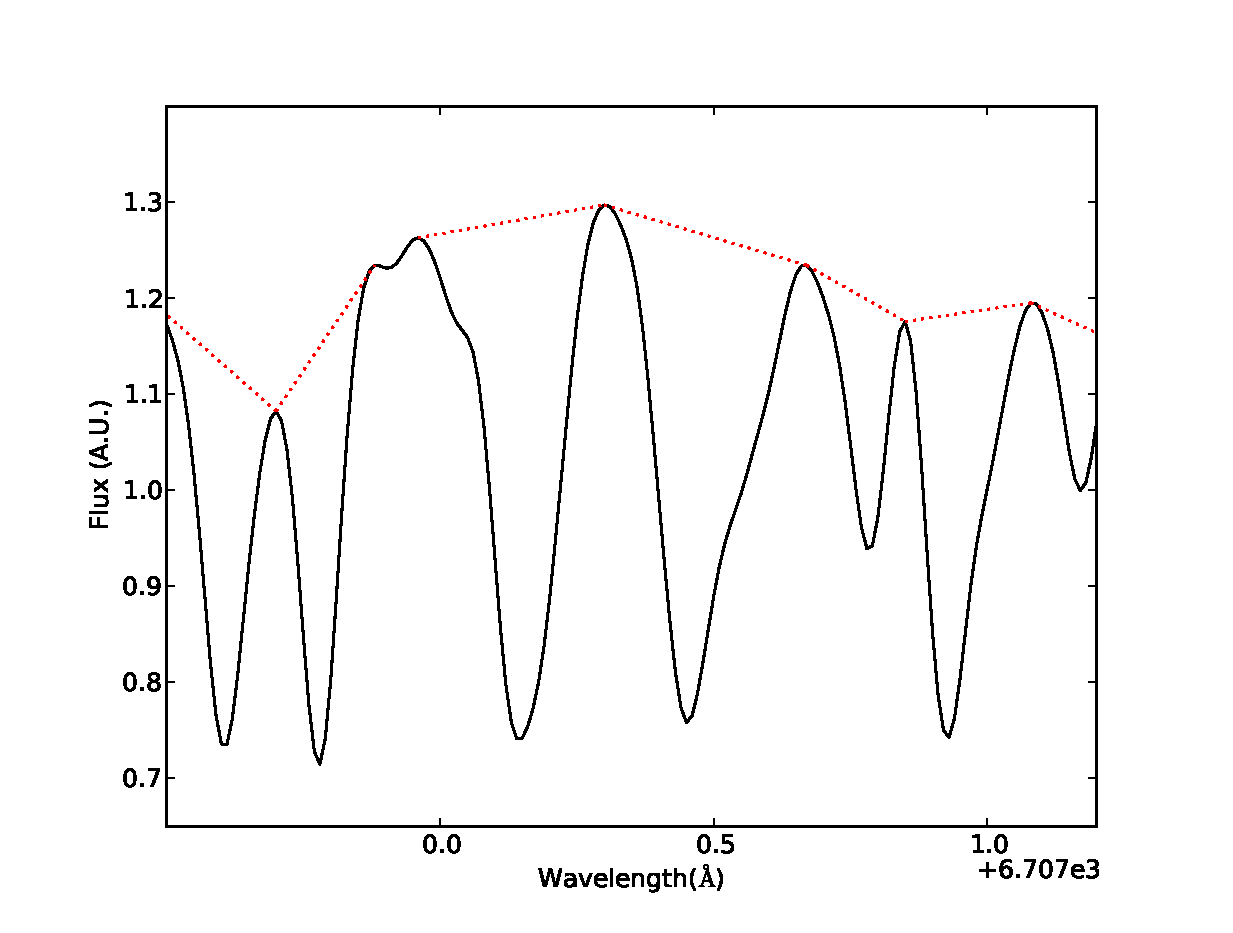
\includegraphics[scale=0.45]{pics/template.eps}
\end{center}
\caption{Small region of the Gl 205 spectra illustrating pseudo equivalent width line measurement. The red dotted line represents the `peak-to-peak' flux.}
\label{fig:spec}
\end{figure}

The next step consisted in the investigation of the correlation between the measured EWs and the reference values for [Fe/H] and $T_{eff}$. Fig. \ref{fig:pcorr} shows the histograms of the partial correlation coefficient values of the EWs with the value of the metallicity and effective temperature (solid blue and dashed green lines respectively). The partial correlation coefficient is defined as the correlation coefficient of one parameter keeping the other fixed. %For the partial correlation of [Fe/H] with EW, for instance, we can write, 
%\begin{equation}
%\rho_{EW,[Fe/H];T_{eff}} = - \frac{\rho_{EW,[Fe/H]}\rho_{T_{eff},T_{eff}}}{\sqrt{(1-\rho_{EW,T_{eff}})(1-\rho_{[Fe/H],T_{eff}}}}
%\end{equation}
We observe, in Fig. \ref{fig:pcorr} that a significant amount of lines have good correlation values with the parameters. 



\begin{figure}[h]
\begin{center}
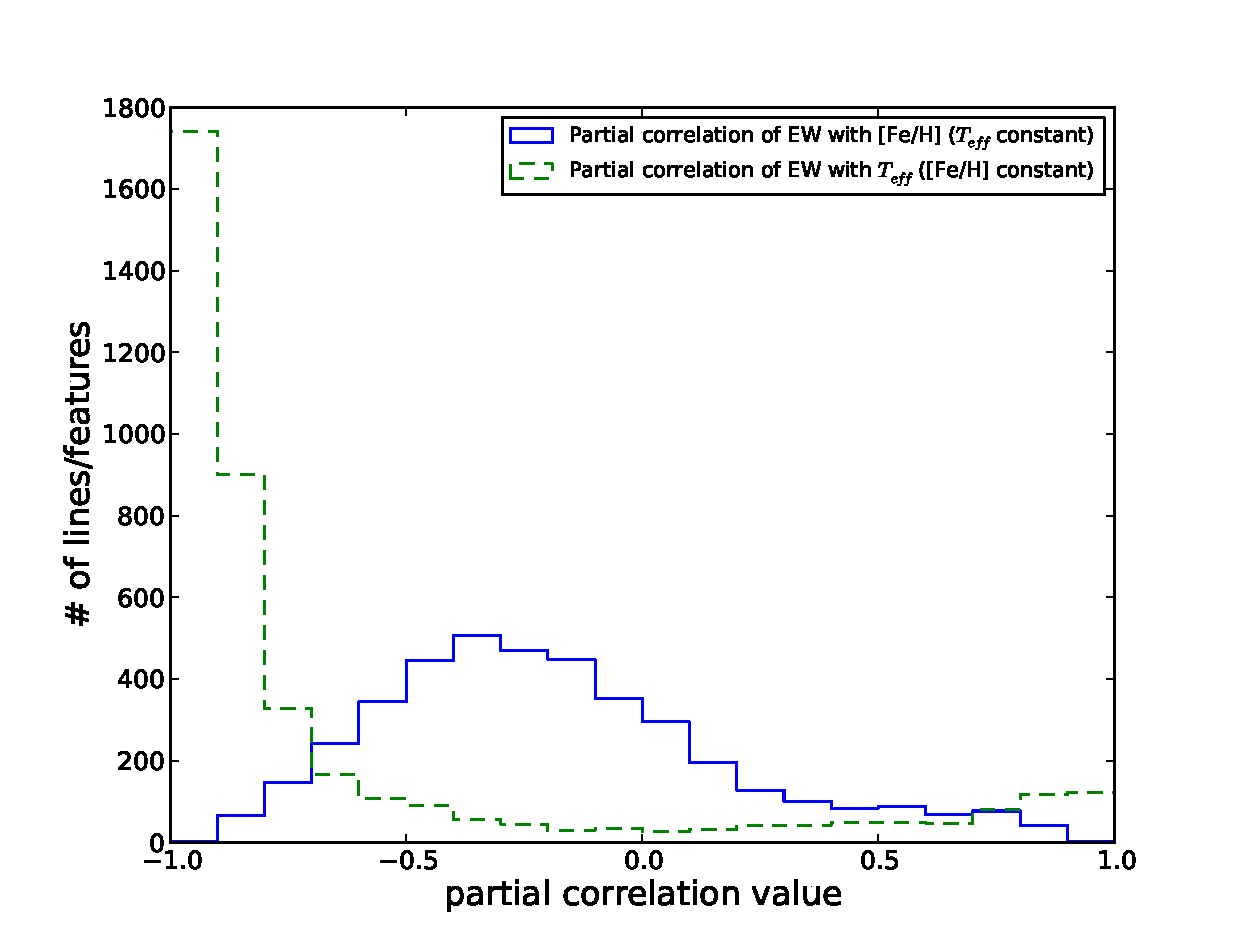
\includegraphics[scale=0.45]{pics/pcorrv2.eps}
\end{center}
\caption{Histograms of the partial correlations of [Fe/H] (solid blue histogram) and $T_{eff}$ (dashed green histogram).}
\label{fig:pcorr}
\end{figure}

At this stage, we discarded three stars  (Gl388, Gl729, Gl803) that were showing bad correlations with either or both the reference metallicity and effective temperature. The cause for the bad correlation is probably due to high activity/rotation. Indeed, the three stars are shown as active in \citet{Bonfils-2013}. This effect is especially visible in the effective temperature of these stars, where its value is much lower than the reference temperature. For Gl388 and Gl729 \citet{Reiners-2012} show that these stars have a very low photometric period (2.2 and 2.9 days respectively) and are very active ($\log{L_{H_{\alpha}}/L_{bol}}$ of -3.8 and -3.77 respectively) despite having a low value of $v\sin{i}$. Gl803, on the other hand is a very young star (20 Myr) with a circumstellar disk \citep{Kalas-2004}. Therefore, it belongs in the same `high rotation/low $v\sin{i}$' group as the other two stars. Our final sample has 58 stars, as shown in Table \ref{table:params}. 

Then we did a least squares linear fit of the EWs with the metallicity and effective temperature. The reference values were calculated with the calibration of \citet{Neves-2012}, for [Fe/H], and with the three ($V-J$, $V-H$, and $V-K_{S}$) photometric calibrations of \citet{Casagrande-2008}, for $T_{eff}$, where we took the average value. From each line/feature $i$ of every star $m$ we calculate a EW value. Then we have

\begin{equation}
W_{i,m} = \alpha_{i}[Fe/H]_{m}^{T} + \beta_{i}T_{eff,m}^{T} + \gamma_{i}, %Ones_{m}^{T},
\label{eq:fit}
\end{equation}

where $W_{i,m}$ is a $i\times m$ matrix containing the EWs, and both $[Fe/H]_{m}^{T}$, and $T_{eff m}^{T}$ are the transpose matrices of the parameter values and are, therefore, $1\times m$ vectors. The $\alpha$ and the $\beta$ are the coefficients related to metallicity and effective temperature, respectively, while $\gamma$ is an independent coefficient. The error associated to each parameter $p$ is calculated as 
%put here reference of MINPACK1 if needed J J More mas basicamente e propagacao de erros
\begin{equation}
\label{eq:rss}
\epsilon_{p} = \sqrt{RSS.J},
\end{equation}
where RSS is the residual sum of squares, expressed as

\begin{equation}
RSS = \frac{\sum{(x_{i,model}-x_{i})^{2}}}{n_{obs}-n_{coef}},
\end{equation}
and $J$ is the diagonal of the estimate of the jacobian matrix around the solution. %The product of the residual sum of squares with the jacobian matrix is an estimate of the covariance matrix of the parameters. 
The $x_{i,model}$, $x_{i}$, $n_{obs}$, and $n_{coef}$ from Eq. \ref{eq:rss} are, respectively, the predicted value of the data, $x_{i}$, by the regression model, the data values, the number of data points, and the number of coefficients. We assume that both metallicity and effective temperature are independent and do not correlate with each other. This assumption was tested by perturbing each parameter in turn by introducing an positive or negative offset and then calculating both parameters. There was no difference in the obtained values of the unperturbed parameter. We also tried to use the full covariance matrix to calculate the uncertainties but in the end we got a worse result for the dispersion of the calibration. Therefore, we decided to use only the diagonal values of the covariance matrix. The total error of the coefficients associated to each line $i$ can then be written as

\begin{equation} 
\epsilon_{i} = \sqrt{\epsilon_{\alpha}^{2}+\epsilon_{\beta}^{2}+\epsilon_{\gamma}^{2}}.
\end{equation}

The aim of the calibration is to increase the precision of both [Fe/H] and $T_{eff}$ determinations. To do that we need to obtain the values of the metallicity and effective temperature via a weighted least squares refit, that is obtained after a left multiplication of $(C^{T}_{3,i}C_{i,3})^{-1}C^{T}_{3,i}$ on both terms of Eq. \ref{eq:fit}, where $C$ is the calibration matrix or the coefficient matrix, that can be written as
\begin{equation}
C_{i,3} = \left[\begin{array}{ccc} \alpha_{1,1} & \beta_{1,2} & \gamma_{1,3} \\ \alpha_{2,1} & \beta_{2,2} & \gamma_{2,3} \\... & ... & ...\\ \alpha_{i,1} & \beta_{i,2} & \gamma_{i,3} \end{array}\right],
\end{equation}
and $C^{T}$ is the transpose of $C$. The refit is then expressed, for each star $m$, as

\begin{equation}
\label{eq:refit}
\left[\begin{array}{c} [Fe/H] \\T_{eff} \\ Ind \end{array}\right] =  (C^{T}_{3,i}C_{i,3})^{-1}C^{T}_{3,i}W_{i,m},
\end{equation}
where $Ind$ is the value of the independent parameter. Finally we introduce a weight to Eq. \ref{eq:refit}, using a \textit{Levenberg-Marquardt} \citep[][]{Press-1992} algorithm. The normalised weight $E_{i}$ is defined as


%Then we invert Eq. \ref{eq:fit}. After some operations we obtain

%\begin{equation}
%[[Fe/H],Teff,Ind]_{3,m} = (C^{T}_{3,i}C_{i,3})^{-1}C^{T}_{3,i}W_{i,m},
%\label{eq:refit}
%\end{equation}

\begin{equation}
E_{i} = \frac{1/\epsilon_{i}^{2}}{\sum{1/\epsilon_{i}^{2}}}.
\label{eq:weight}
\end{equation}

Other methods were tested, such as choosing lines/features with the best correlations or partial correlations with the parameters. However, the weighted least squares approach performed best at minimising the uncertainties of both metallicity and temperature. 

Quantitatively we obtain a dispersion of 0.07 dex for the metallicity and 100K for the effective temperature, as shown in Fig. \ref{fig:fehfeh}. The calibration is valid between -0.91 to 0.25 dex for [Fe/H], 2600 to 3800 K for $T_{eff}$, and between M0 to M5.5, considering a $\pm$ 0.5 uncertainty in the spectral type. Our dispersion is described by the root mean square error (RMSE), and defined as

\begin{equation}
RMSE = \sqrt{\frac{\sum{(x_{i}-x_{ref})^{2}}}{n_{obs}-n_{coef}}},
\end{equation}
where $x_{i}$ is the estimated quantity, $x_{ref}$ the reference value for the same quantity, $n_{obs}$ the number of calibrators and $n_{coef}$ the number of parameters used in the calibration (three in this case). 

The calculated parameters as well as the reference determinations for [Fe/H] and $T_{eff}$ are listed in Table \ref{table:cal}. Columns 1 and 3 contain the values for the reference calibrations, while columns 2 and 4 show the values obtained with our new calibration. We emphasise here that we only get an improvement on the precision. The accuracy of the calibration as well as its systematics are tied to the original determinations of the parameters. %\textcolor{red}{check the precisions and the plots}

\begin{figure*}[t!]
\begin{center}
\subfigure[]{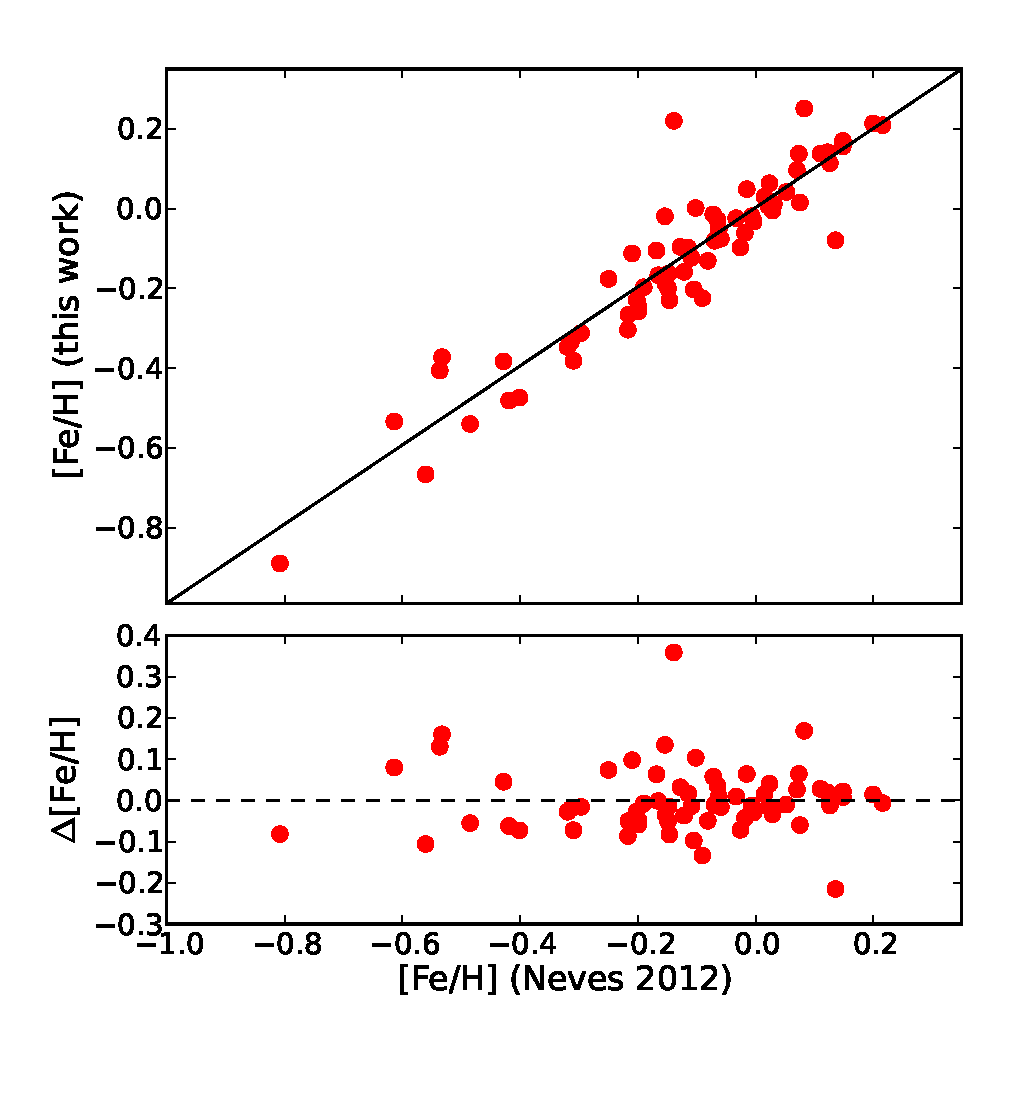
\includegraphics[scale=0.54]{pics/fehfehn12v2.eps}}
\subfigure[]{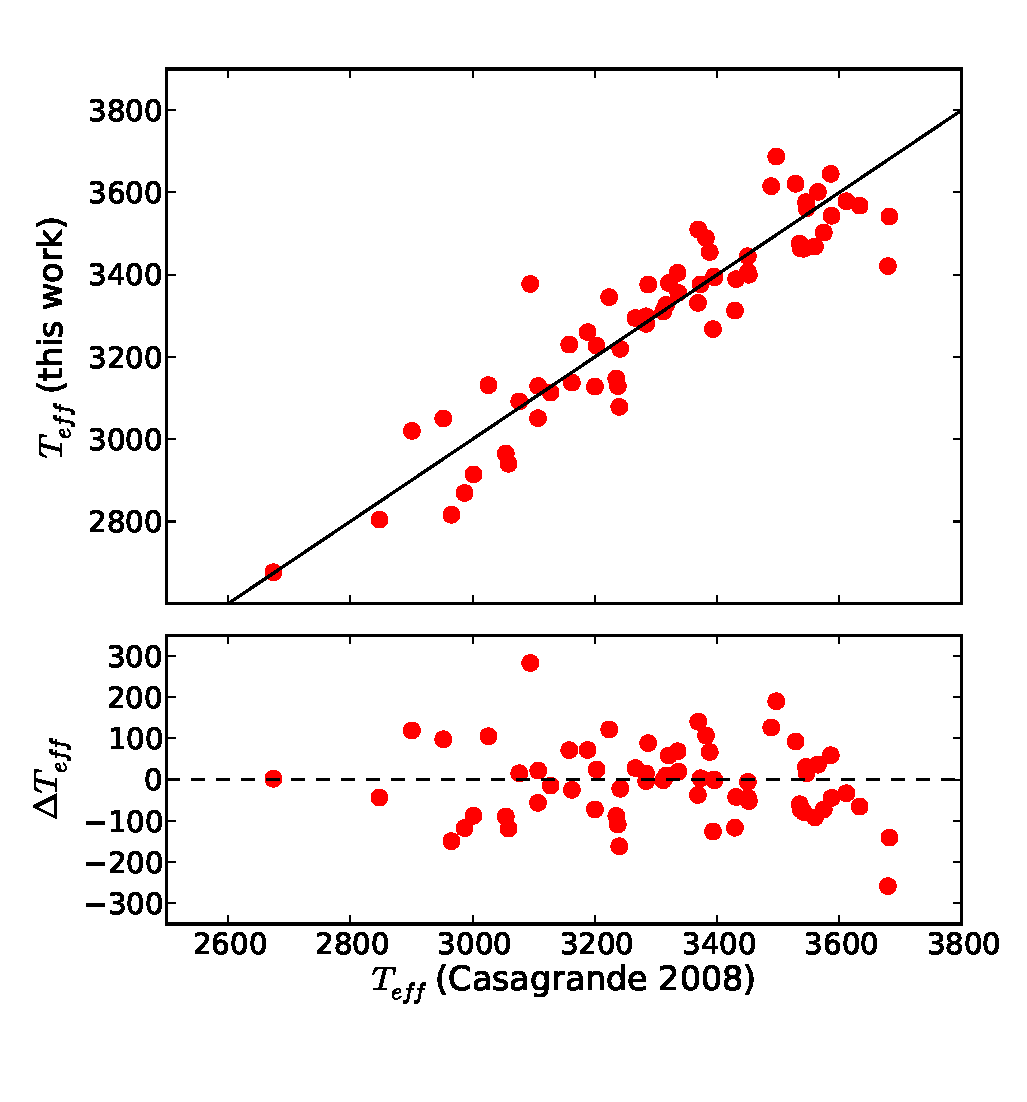
\includegraphics[scale=0.54]{pics/teffteffc08v2.eps}}
\end{center}
\caption{(a) [Fe/H] comparison between this work and the photometric calibration of \citet{Neves-2012}; (b) $T_{eff}$ comparison between this work and the photometric calibration of \citet{Casagrande-2008}.}
\label{fig:fehfeh}
\end{figure*}
%
%

\begin{table}[t!]
\caption{ Calibration sample table with the reference and calibrated metallicity and effective temperature. Sorted by right ascension.}
\label{table:cal}
\begin{tabular}{ l r r r r}
\hline
\hline
star & [Fe/H]$_{N12}$ & [Fe/H]$_{NEW}$ & $T_{eff C08}$ & $T_{eff NEW}$ \\
       &         [dex]          &      [dex]              &[       [K]                &  [K] \\
\hline
Gl1 & -0.42 & -0.48 & 3528 & 3612 \\
Gl54.1 & -0.43 & -0.40 & 2901 & 2997 \\
Gl87 & -0.32 & -0.34 & 3565 & 3601 \\
Gl105B & -0.15 & -0.04 & 3054 & 2958 \\
LP771-95A & -0.53 & -0.38 & 3393 & 3261 \\
Gl176 & -0.00 & -0.01 & 3369 & 3355 \\
Gl191 & -0.81 & -0.91 & 3679 & 3389 \\
Gl205 & 0.15 & 0.25 & 3497 & 3768 \\
Gl213 & -0.21 & -0.13 & 3026 & 3120 \\
Gl229 & -0.06 & 0.01 & 3586 & 3700 \\
HIP31293 & -0.06 & -0.07 & 3312 & 3319 \\
HIP31292 & -0.13 & -0.10 & 3158 & 3236 \\
Gl250B & -0.11 & -0.10 & 3369 & 3526 \\
Gl273 & -0.07 & -0.04 & 3107 & 3122 \\
Gl300 & 0.07 & 0.11 & 2965 & 2809 \\
GJ2066 & -0.11 & -0.19 & 3388 & 3466 \\
Gl341 & -0.17 & -0.11 & 3633 & 3613 \\
GJ1125 & -0.17 & -0.12 & 3162 & 3134 \\
Gl357 & -0.31 & -0.33 & 3335 & 3406 \\
Gl358 & -0.01 & -0.02 & 3240 & 3088 \\
Gl367 & -0.11 & -0.08 & 3452 & 3418 \\
Gl382 & 0.02 & 0.04 & 3429 & 3348 \\
Gl393 & -0.15 & -0.22 & 3396 & 3409 \\
Gl413.1 & -0.08 & -0.11 & 3373 & 3395 \\
Gl433 & -0.15 & -0.17 & 3450 & 3472 \\
Gl438 & -0.54 & -0.39 & 3536 & 3475 \\
Gl447 & -0.25 & -0.20 & 2952 & 3036 \\
Gl465 & -0.56 & -0.67 & 3382 & 3467 \\
Gl479 & 0.03 & -0.00 & 3238 & 3143 \\
Gl514 & -0.15 & -0.15 & 3574 & 3537 \\
Gl526 & -0.20 & -0.23 & 3545 & 3583 \\
Gl536 & -0.15 & -0.13 & 3546 & 3586 \\
Gl551 & 0.08 & -0.01 & 2674 & 2649 \\
Gl555 & 0.11 & 0.11 & 2987 & 2865 \\
Gl569A & 0.14 & -0.06 & 3235 & 3165 \\
Gl581 & -0.20 & -0.24 & 3203 & 3232 \\
Gl588 & 0.05 & 0.05 & 3284 & 3320 \\
Gl618A & -0.07 & -0.08 & 3242 & 3227 \\
Gl628 & -0.06 & -0.05 & 3107 & 3050 \\
Gl667C & -0.48 & -0.54 & 3431 & 3388 \\
Gl674 & -0.20 & -0.26 & 3284 & 3285 \\
Gl678.1A & -0.12 & -0.10 & 3611 & 3623 \\
Gl680 & -0.09 & -0.20 & 3395 & 3411 \\
Gl682 & 0.07 & 0.07 & 3002 & 2907 \\
Gl686 & -0.31 & -0.36 & 3542 & 3476 \\
Gl693 & -0.30 & -0.32 & 3188 & 3251 \\
Gl699 & -0.61 & -0.55 & 3094 & 3356 \\
Gl701 & -0.22 & -0.27 & 3535 & 3497 \\
Gl752A & 0.01 & 0.04 & 3336 & 3376 \\
Gl832 & -0.19 & -0.18 & 3450 & 3430 \\
Gl846 & -0.10 & 0.08 & 3682 & 3613 \\
Gl849 & 0.22 & 0.20 & 3200 & 3143 \\
Gl876 & 0.12 & 0.11 & 3059 & 2939 \\
Gl877 & -0.03 & -0.03 & 3266 & 3304 \\
Gl880 & 0.03 & 0.07 & 3488 & 3666 \\
Gl887 & -0.22 & -0.24 & 3560 & 3491 \\
Gl908 & -0.40 & -0.47 & 3587 & 3534 \\
LTT9759 & 0.15 & 0.18 & 3316 & 3354 \\
\hline
\hline
\end{tabular}
%\hline
\end{table}











%Column 1 shows the star designation, column 2 the reference photometric calibration, column 3 the calibrated [Fe/H] value, column 4 the initial photometric $T_{eff}$, and column 5 the calibrated effective temperature




\subsection{Estimation of the calibration uncertainties}

To validate our calibration and have a better understanding of the uncertainties of our measurements we performed a bootstrap resampling and calculated the root mean square error of validation (RMSE$_{V}$) of our calibration. 

\begin{figure*}[b!]
\begin{center}
\subfigure[]{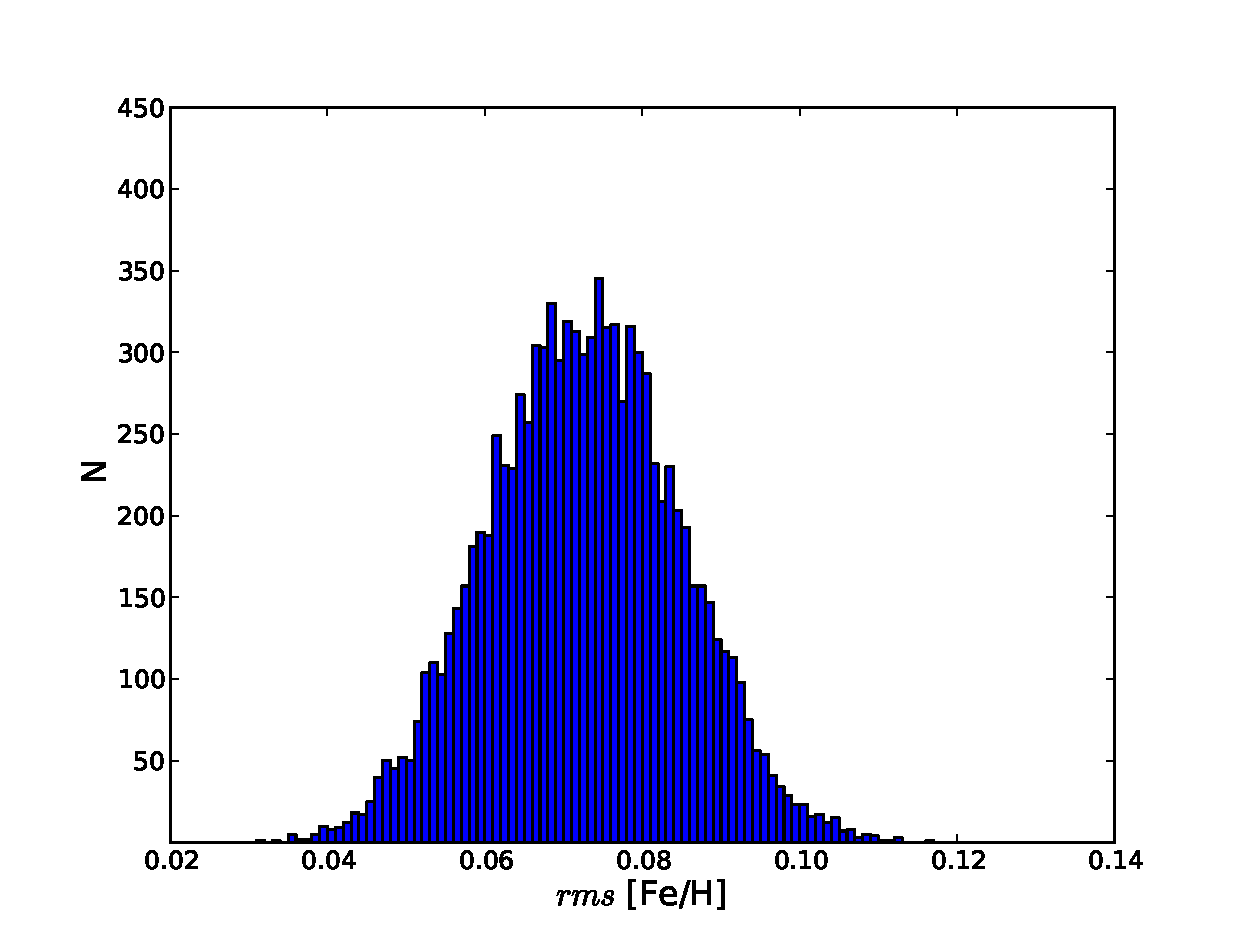
\includegraphics[scale=0.44]{pics/hist_fehv2.eps}}
\subfigure[]{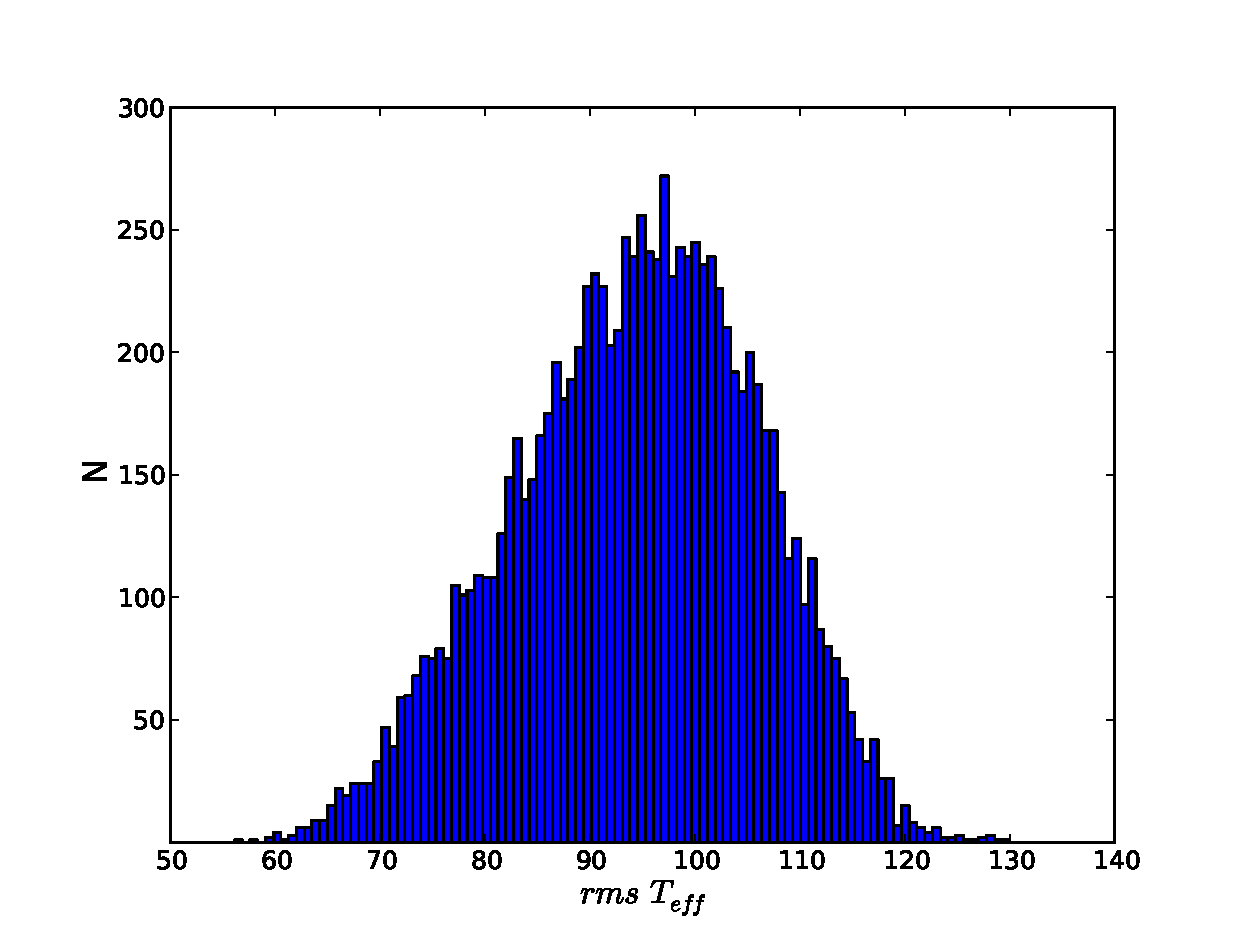
\includegraphics[scale=0.44]{pics/hist_teffv2.eps}}
\end{center}
\caption{Histogram of the dispersion given by bootstrap for [Fe/H] (a) and $T_{eff}$ (b). The N is the number of trials.}
\label{fig:strap}
\end{figure*}

The bootstrap method we implemented tests how the $rms$ of the calibration changes when using slightly different `bootstrapped' samples. To have a statistical significative number we first created 10.000 virtual samples by randomly drawing with repetition, for each virtual sample, a number of stars equal to the size of our sample. The random drawing followed a random uniform distribution. Then we calculated the $rms$ for each trial and measured the $1\sigma$ Gaussian equivalent interval between 15.9\% and 84.1\% from the resulting distribution, following the procedure of e.g. \citet{Burgasser-2003,Neves-2013}. The distributions of the $rms$ for both parameters are depicted in Fig. \ref{fig:strap}. The final result shows a variation of the $rms$ of the [Fe/H] and $T_{eff}$ by  $\pm 0.01$ dex and $\pm 13$ K respectively.



The calculation of the RMSE$_{V}$ is a predicted residual sum of squares (PRESS) procedure \citep{Weisberg-2005} and follows the description in the Appendix of \citet{Rojas-Ayala-2012}. In short, we try to obtain the original value of the metallicity and temperature of each star $i$ of the calibration leaving that star out when calculating the calibration. Then, we calculate the residuals, or the difference between the original and obtained value for each star and add them up in quadrature. The PRESS statistic is then defined as 
\begin{equation}
PRESS = \sum{(y_{i}-y_{ref}})^{2},
\end{equation}
where $y_{i}$ is the estimated value of the parameter and $y_{ref}$ is the reference value of the measured quantity. From here we can calculate the root mean squared error of validation,

\begin{equation}
RMSE_{V} = \sqrt{\frac{PRESS}{n_{V}}},
\end{equation}
where $n_{V}$ is the number of calibrators. The RMSE$_{V}$ value can then be used to obtain confidence intervals. We obtain a RMSE$_{V}$ value of 0.08 dex and $\sim$ 300 K for the [Fe/H] and $T_{eff}$ respectively and will use these values as our $1\sigma$ confidence intervals, assuming a normal cumulative distribution function. \textcolor{red}{Discuss last phrase. Babs?}. Table \ref{table:errors} summarises our results. 

\begin{table}[]
\centering
\caption[]{Uncertainty estimators for [Fe/H] and $T_{eff}$.}
\label{table:errors}
%\resizebox{12cm}{!}{
\begin{tabular}{l c c}
\hline
\hline
Estimator & [Fe/H] & $T_{eff}$ \\ 
                &  [dex]  &  [K] \\
\hline
RMSE & 0.07 & 100\\
Bootstrap & 0.07$\pm$0.01 & 100$\pm$20 \\
RMSE$_{V}$ & 0.08 & 300 \\
\hline
\hline
\end{tabular}
\end{table}

We observe that the uncertainties calculated with the different techniques are consistent with each other. The uncertainty for $T_{eff}$ is large but is in line with the expected uncertainties. We also perturbed our calibration by introducing an offset in [Fe/H] or $T_{eff}$, as explained in Sect. \ref{sec:method}. We concluded that an introduction of a fixed quantity on either parameter does not affect the measurement of the other.   %of synthetic spectra modelling \textcolor{red}{ref?????, private comm from Christiane Helling or France Allard is enough?}.

\subsection{Testing the calibration as a function of resolution and SNR}

We also calculated the dispersion of the parameters as a function of the resolution and SNR. The resolution of the HARPS spectra was degraded by means of a convolution between the spectra and a normalised gaussian curve, simulating the instrumental profile, with $FWHM = \lambda/R$, where $\lambda$ is the wavelength and $R$ the resolution we intend to obtain. %The $5500 \AA$  is the wavelength we chose as reference. 
From here, the standard deviation of the gaussian is calculated with the well known formula 

\begin{equation}
\label{eq:fwhm}
\sigma = \frac{FWHM}{2\sqrt{2\log{2}}}. 
\end{equation}

The desired signal to noise ratio was obtained by introducing random gaussian noise in the spectra. The $\sigma$ and the noise were adjusted to the HARPS resolution ($R\sim115.000$) and to the original SNR @ $5500 \AA$  of each spectrum \textcolor{red}{Should we use here a longer wavelength reference?}. The final values for both parameters are


%, where the maximum value \textcolor{red}{(maximum or 1-sigma???} of the injected noise is defined as 

%\begin{equation}
%noise = \frac{1}{SNR}, 
%\end{equation}
%where SNR is the value we want to obtain. 


\begin{equation}
\sigma' = \sqrt{\sigma^2-\sigma_{HARPS}^2},
\end{equation}
and
\begin{equation}
noise' = \sqrt{noise^{2} - noise_{HARPS}^{2}}.
\end{equation}

Figures \ref{fig:resnr-feh} and \ref{fig:resnr-teff} show the residuals as a function of resolution (while SNR is kept constant at 100) and as a function of SNR (while the resolution is kept constant at 100.000) for [Fe/H] and $T_{eff}$ respectively. The red dotted line depicts the offset of the residuals. 

\begin{figure*}[h!]
\begin{center}
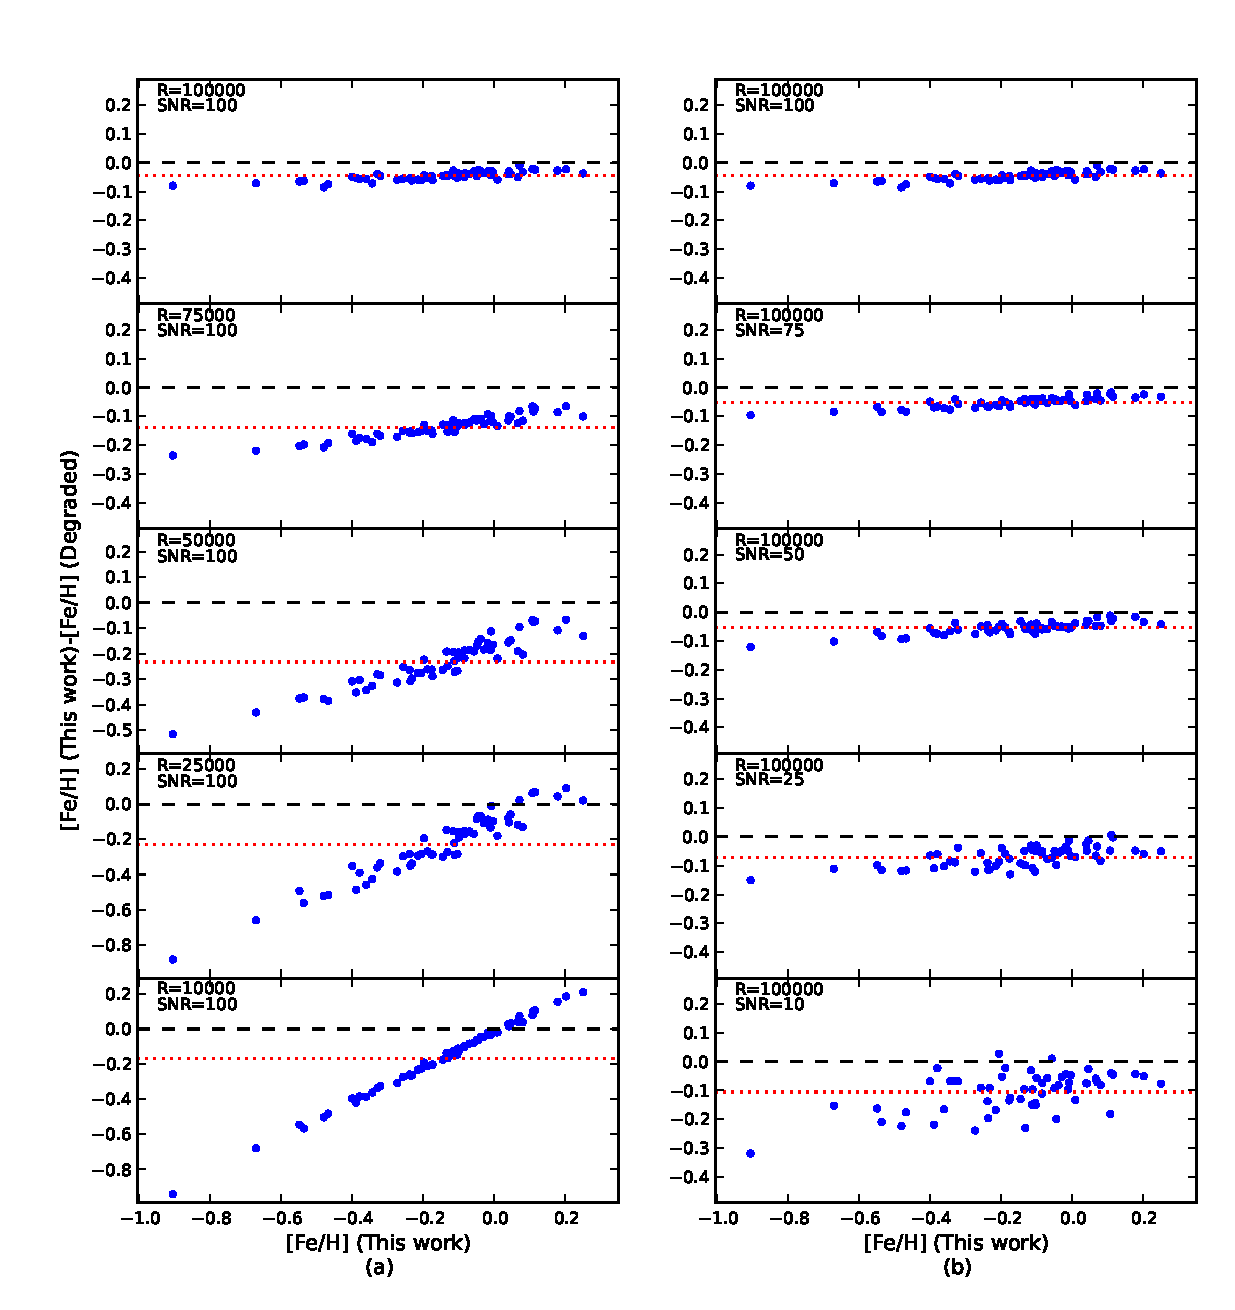
\includegraphics[scale=0.9]{pics/resnr_feh.eps}
\end{center}
\caption{Difference of the [Fe/H] for this work and the [Fe/H] calculated with different resolution/SNR combinations as a function of the resolution and SNR.}
\label{fig:resnr-feh}
\end{figure*}

\begin{figure*}[h!]
\begin{center}
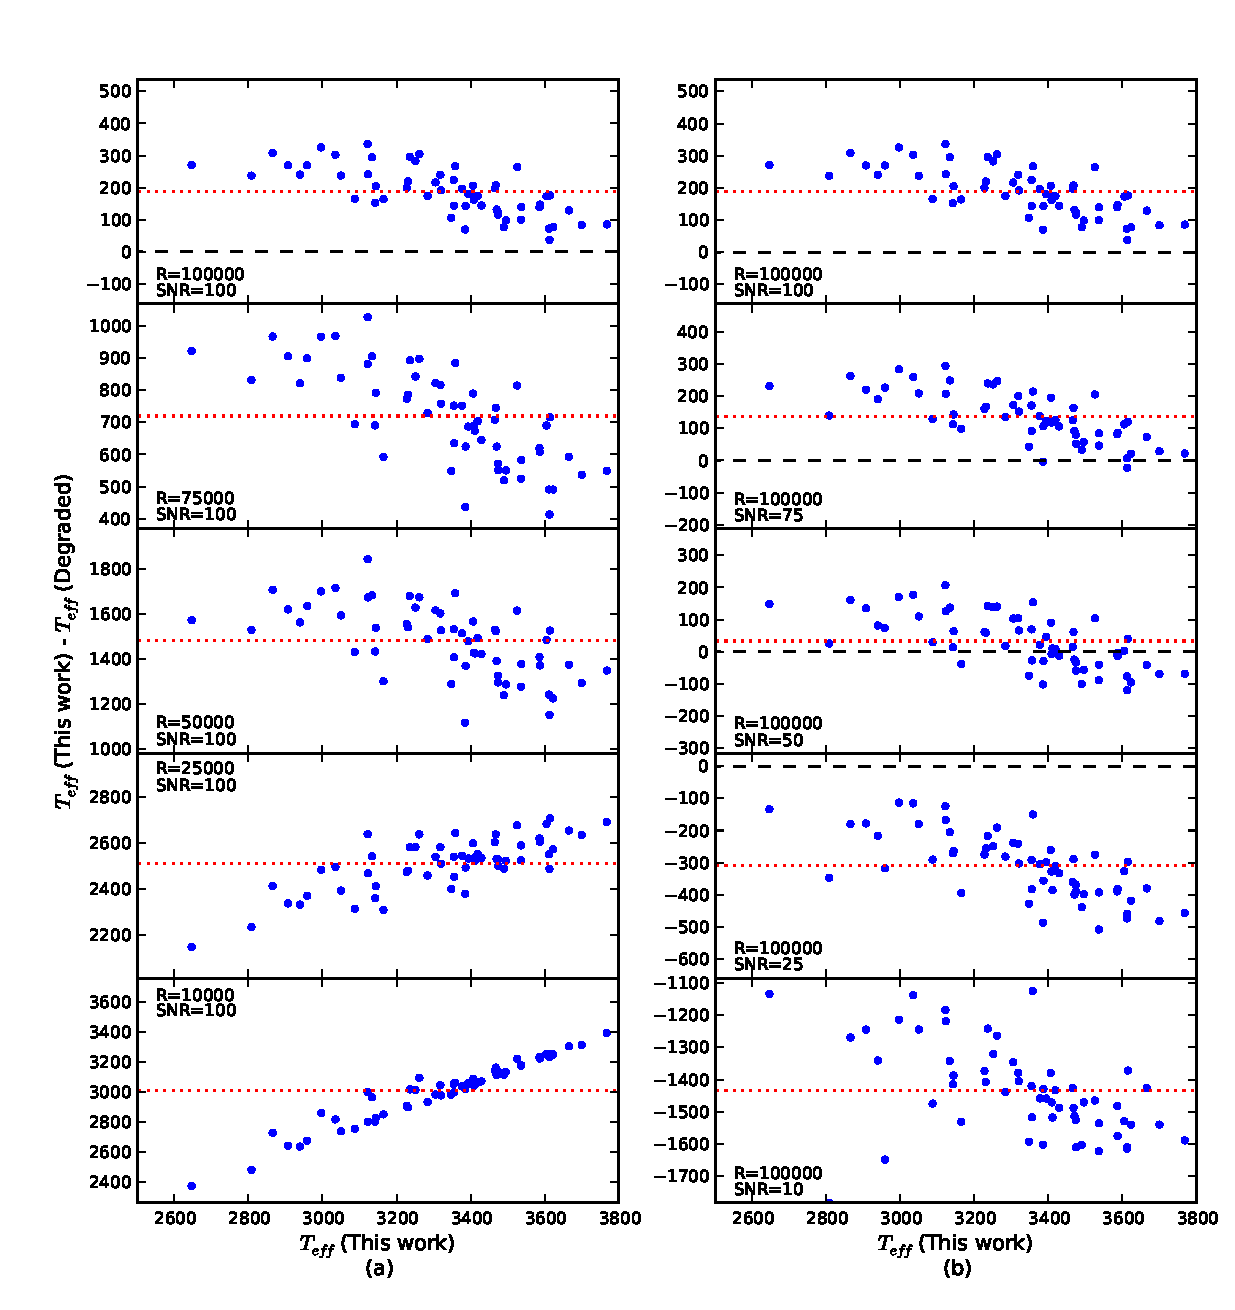
\includegraphics[scale=0.9]{pics/resnr_teff.eps}
\end{center}
\caption{Difference of the [Fe/H] for this work and the [Fe/H] calculated with different resolution/SNR combinations as a function of the resolution and SNR.}
\label{fig:resnr-teff}
\end{figure*}


We observe in both Figures the existence of different trends for different resolutions and SNR. To correct these trends we performed a linear fit for each Resolution/SNR combination with the functional form [Fe/H](This work)$ = a.$[Fe/H](Degraded)+$b$ for metallicity, and 
$T_{eff}$(This work)$ = a.T_{eff}$(Degraded)+$b$ for effective temperature. The values for each combination are shown in Table \ref{table:linfit}. 

\begin{table*}[t!]
\begin{center}
\caption{Linear fit coefficients $a$ and $b$ from the relation between the values of the parameters of this work calibration and the values calculated for different combinations of resolution and SNR.  }
\label{table:linfit}
\subtable[{[Fe/H]}]{
%\resizebox{9cm}{!}{
\begin{tabular}{l | r r | r r | r r | r r | r r}
\hline
\hline
SNR & \multicolumn{2}{c|}{100} & \multicolumn{2}{c|}{75} & \multicolumn{2}{c|}{50} & \multicolumn{2}{c|}{25} & \multicolumn{2}{c}{10} \\
Resolution & a & b & a & b & a & b & a & b & a & b \\
\hline
100000 & 1.0582 & -0.0394 & 1.0705 & -0.0443 & 1.0796 & -0.0471 & 1.0956 & -0.0624 & 1.0910 & -0.1013 \\
75000 & 1.1894 &  -0.1353 & 1.2101 & -0.1362 & 1.2113 & -0.1396 & 1.2727 & -0.1520 & 1.1727 & -0.1749 \\
50000 & 1.5908 &  -0.2804 & 1.6063 & -0.2848 & 1.6390 & -0.2843 & 1.6140 & -0.2792 & 1.3489 & -0.2667 \\
25000 & 1.9301 &  -0.3021 & 1.8556 & -0.2900 & 1.7552 & -0.2787 & 1.7526 & -0.2667 & 0.9696 & -0.2119 \\
10000 & 0.7717 &  -0.1656 & 1.3339 & -0.1747 & 2.0107 & -0.1881 & 1.0431 & -0.1774 & 0.7522 & -0.1860 \\
\hline
\end{tabular}
}

\subtable[$T_{eff}$]{
%\caption{$T_{eff}$}
\begin{tabular}{l | r r | r r | r r | r r | r r}
\hline
\hline
SNR & \multicolumn{2}{c|}{100} & \multicolumn{2}{c|}{75} & \multicolumn{2}{c|}{50} & \multicolumn{2}{c|}{25} & \multicolumn{2}{c}{10} \\
Resolution & a & b & a & b & a & b & a & b & a & b \\
\hline
100000 & 0.7957 &  829.0747 & 0.7865 & 818.5115 & 0.7764 & 769.6886 & 0.7312 & 667.9319 & 0.6666 & 152.6770 \\
75000 &   0.6336 & 1674.7330 & 0.6389 & 1624.5838 & 0.6454 & 1526.6327 & 0.6485 & 1265.5323 & 0.6181 & 618.0058 \\
50000 &   0.6284 & 2165.7729 & 0.6511 & 2081.6257 & 0.6667 & 1955.7645 & 0.6979 & 1581.2159 & 0.6813 & 740.3490 \\
25000 &   1.2686 & 2292.4712 & 1.3430 & 2120.1743 & 1.3703 & 1864.6764 & 1.2981 & 1279.5182 & 1.0348 & 222.7126 \\
10000 &   2.2880 & 2601.2130 & 3.5903 & 1815.5954 & 3.2029 & 1357.7898 & 1.2830 & 1835.07950 & 0.6124 & 1713.3062 \\
\hline
\end{tabular}}

\end{center}
\end{table*}

From here we calculated the dispersion of the difference between the corrected parameter values and the ones obtained from our original calibration, and added this dispersion with the one from our calibration in quadrature. Table \ref{table:snres} shows the results. The horizontal header of both tables correspond to the SNR of the spectra, between 100 and 10,  while the vertical header depicts their resolution, from 100.000 to 10.000. The row with the resolution number is the value of the dispersion of the calibration using the corresponding resolution/snr combination. The rows with the suffix $res$ show the dispersion of the difference between the values of our calibration and the ones obtained with the corrected values for each resolution/snr combination.

\begin{table}[t!]
\begin{center}
\caption{Dispersion of the residuals of the parameters as a function of the resolution and SNR. }
\label{table:snres}
\subtable[{[Fe/H]}]{
%\resizebox{9cm}{!}{
\begin{tabular}{l r r r r r }

\hline
\hline
SNR & 100 & 75 & 50 & 25 & 10 \\
Resolution &    &   &     &       & \\
\hline
100000 & 0.071 & 0.071 & 0.071 & 0.076 & 0.098 \\
100000res & 0.010 & 0.010 & 0.013 & 0.030 & 0.068 \\
75000 & 0.072 & 0.073 & 0.073 & 0.082 & 0.110 \\
75000res & 0.016 & 0.020 & 0.021 & 0.043 & 0.085 \\
50000 & 0.087 & 0.092 & 0.100 & 0.113 & 0.140 \\
50000res & 0.052 & 0.060 & 0.072 & 0.089 & 0.121 \\
25000 & 0.202 & 0.206 & 0.207 & 0.204 & 0.219 \\
25000res & 0.189 & 0.194 & 0.195 & 0.192 & 0.207 \\
10000 & 0.235 & 0.235 & 0.233 & 0.233 & 0.230 \\
10000res & 0.224 & 0.224 & 0.222 & 0.222 & 0.219 \\
\hline
\end{tabular}}

\subtable[$T_{eff}$]{
\begin{tabular}{l r r r r r }
\hline
\hline
SNR & 100 & 75 & 50 & 25 & 10 \\
Resolution &    &   &     &       & \\
\hline
100000 & 109 & 110 & 112 & 114 & 136 \\
100000res & 43 & 45 & 51 & 55 & 92 \\
75000 & 121 & 120 & 121 & 124 & 142 \\
75000res & 68 & 66 & 68 & 73 & 101 \\
50000 & 132 & 130 & 131 & 135 & 147 \\
50000res & 86 & 83 & 84 & 91 & 108 \\
25000 & 148 & 145 & 146 & 163 & 192 \\
25000res & 109 & 105 & 106 & 129 & 164 \\
10000 & 219 & 207 & 226 & 255 & 256 \\
10000res & 195 & 181 & 203 & 235 & 236 \\
\hline
\end{tabular}}
%}
\end{center}
\end{table}


From Table \ref{table:snres} and Figs. \ref{fig:resnr-feh} and \ref{fig:resnr-teff} we observe that, as the resolution degrades, the dispersion and offset of the residuals increase. In the case of [Fe/H], the dispersion value holds well for resolution and SNR higher and equal to 50.000 and 25, respectively.% In the case where $R=50.000$ the calibration might be used if the offset is taken into account. 
Below $R = 50.000$ we consider that the calibration has a value of dispersion that is too high and therefore cannot be applied. Regarding T$_{eff}$, we consider that the calibration is valid for the same resolution and SNR intervals as in [Fe/H]. %However, we note that the dispersion of the T$_{eff}$, after the offset correction, is slightly higher than the dispersion of the original sample at $R=100.000$ but then increases very fast with decreasing resolution. Nevertheless we consider that the dispersion for $T_{eff}$ is valid down to $R=50.000$. 
Table \ref{table:snres} may be used as a guideline for the uncertainties of the parameters when using spectra other than HARPS. %We recommend to use 
%that the offset is always corrected so that the obtained values are the best possible. 
The increasing dispersions and offsets with the resolution should originate from the nature of our `peak-to-peak technique' because it does not consider the continuum. As the resolution gets worse, more and more flux from the `peak to peak' region is lost to the line wings. Moreover, as the resolution decreases there is an increase of line blending that makes the measurement of the correct flux of the each line/feature increasingly difficult.

%To this end we can use the two-sided t-student distribution with $n-p = 52$ degrees of freedom, where $n$ is the number of calibrators and $p$ the number of parameters of the calibration.  



\section{Comparison with the literature}
\label{sec:comp}
A comparison with other studies in the literature was performed. This comparison allow us to have a measure of the accuracy of our calibration and the possible systematics that it may suffer. The results are shown in Table \ref{table:comp}. The results for [Fe/H] are separated by photometric and spectroscopic techniques. The first column depicts the name of the calibration along with its reference. Column two and three describe the dispersion and offset. The last column reports the number of stars in common with our sample. 

\begin{table}[h]
\centering
\caption[]{Dispersion and offset of [Fe/H] and $T_{eff}$ from the residuals of our calibration against other studies. The last column shows the number of stars in common. }
\label{table:comp}
\begin{center}
%\resizebox{12cm}{!}{
\begin{tabular}{l r r r}
\hline
\hline
Photometric [Fe/H] calibrations  &  $rms$  & offset  &  N \\
\hline
B05 \citep{Bonfils-2005}  &  0.10 & -0.04 & 58 \\
SL10 \citep{Schlaufman-2010} &  0.11 & 0.03 & 58 \\
J12 \citep{Johnson-2012} &  0.20 & 0.09 & 58 \\
\hline
Spectroscopic [Fe/H] calibrations  &  $rms$  &  offset  &  N \\
\hline
All calibrations &  0.12 & 0.06 & 38 \\
RA12 \citep{Rojas-Ayala-2012}  &  0.12 & 0.05 & 15 \\
\hline
$T_{eff}$ calibrations & $rms$ & offset & N \\
\hline
RA12 \citep{Rojas-Ayala-2012} & 293 & 230 & 15 \\
O12 \citep{Onehag-2012} & 143 & 51 & 6 \\
BO12 \citep{Boyajian-2012}& 161 & 123 & 44 \\
M13b \citep{Mann-2013b} & 150 & 92 & 6 \\
R13 \citep{Rajpurohit-2013a} & 150 & 117 & 9 \\ 
\hline
\hline
\end{tabular}
\end{center}
\end{table}

\begin{figure*}[]
\begin{center}
\subfigure[]{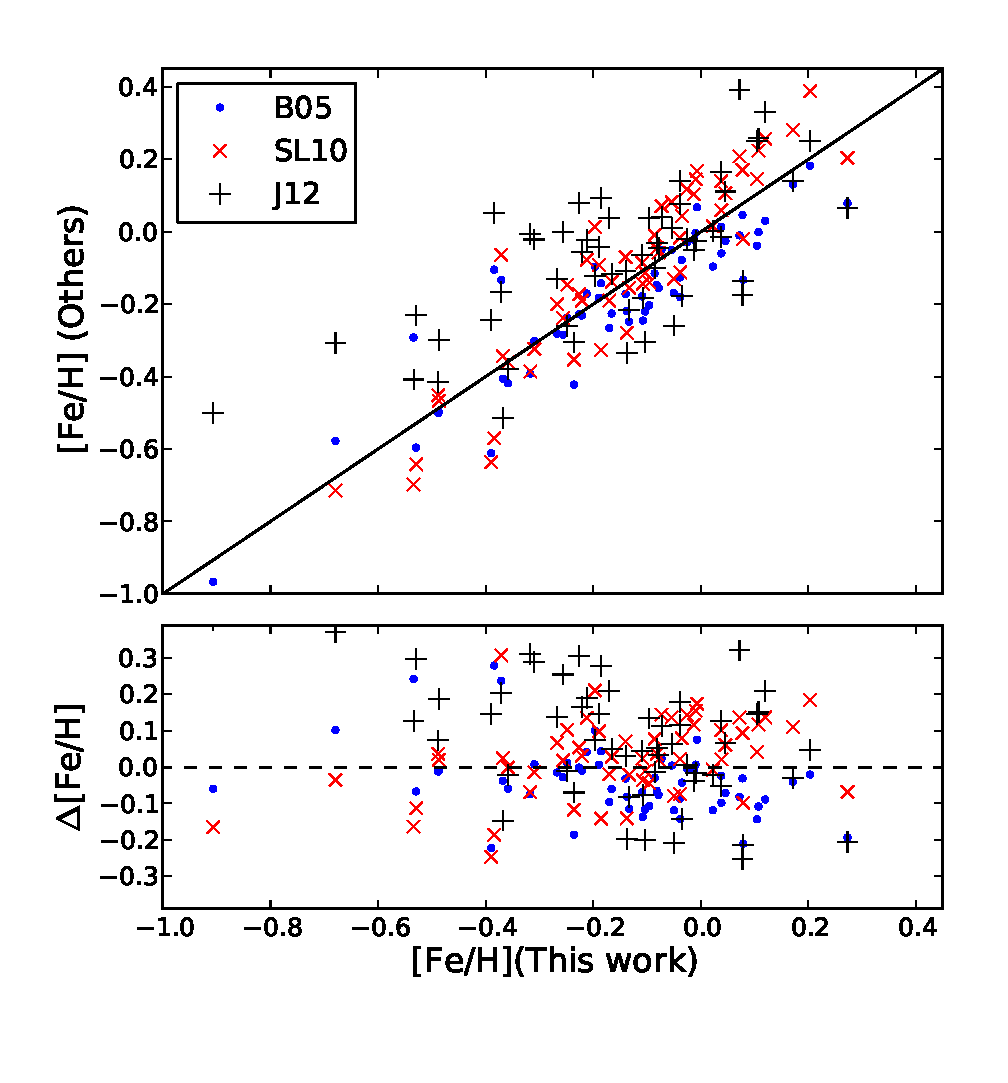
\includegraphics[scale=0.5]{pics/compfehph.eps}}
\subfigure[]{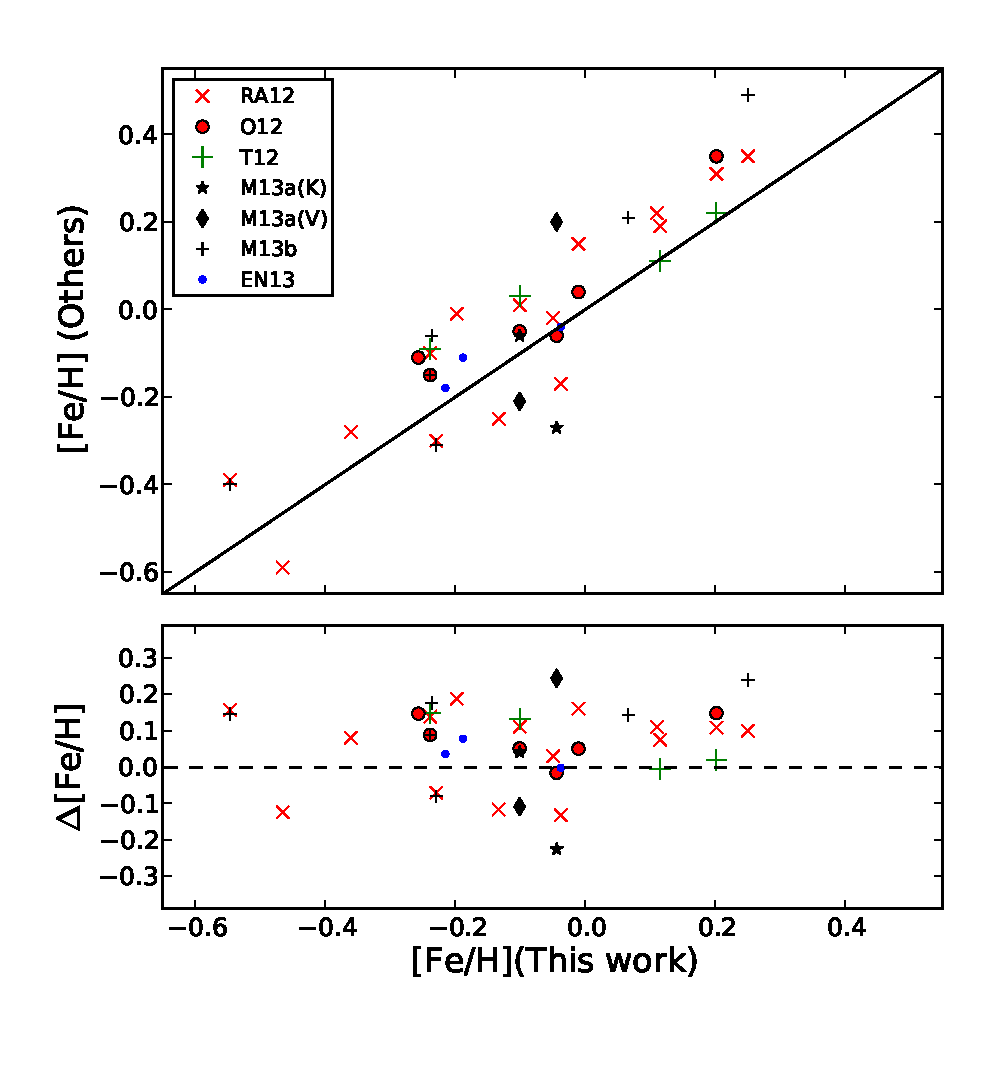
\includegraphics[scale=0.5]{pics/compfehspec.eps}}
\end{center}
\caption{\textit{Upper panel:} [Fe/H]-[Fe/H] plots comparing the values of this work against others in the literature. The plot (a) shows the results of our work versus three photometric calibrations taken from the literature, while plot (b) depicts the comparison between our results against other works.The solid black line of both (a) and (b) depict the identity line;\textit{Lower panel:} Comparison plot residuals. The dashed black line marks the zero point of our calibration.}
\label{fig:compfeh}
\end{figure*}


The photometric [Fe/H] was calculated with the relations of \citet{Bonfils-2005}, \citet{Schlaufman-2010} and \citet{Johnson-2012} (hereafter B05, SL10, and J12, while the spectroscopic [Fe/H] was taken directly from the works of  \citet{Rojas-Ayala-2012}, \citet{Onehag-2012}, \citet{Terrien-2012}, \citet{Newton-2013}, and \citet{Mann-2013b} (hereafter RA12,O12,T12, EN13, and M13b respectively), except in the case of \citet{Mann-2013a} (hereafter M13), where the values of the visible (their Eq. 8) and K-band (their Eq. 16) calibrations were provided directly by the author.



Figure \ref{fig:compfeh} shows two [Fe/H]-[Fe/H] plots. The left plot (a) shows the comparison of our results with the works based on photometric scales. The blue dots, red crosses and black plus signs indicate the results of B05, SL10, and J12 respectively. The right plot (b) depicts the comparison of our work with other spectroscopic calibrations. The red crosses, red circles, green plus signs, black stars, diamonds, and pluses and blue dots correspond to the measurements of RA12, O12, T12, M13, M13b, and EN13 respectively. The (K) and (V) in M13 correspond to measurements performed with a V- and K-band calibration respectively. The solid black line in the upper panel of both plots defines an identity line. The lower panels show the residuals. The dashed black line marks the zero-point of the calibration.

\textbf{Regarding the effective temperature, the photometric temperature scale of \citet{Boyajian-2012} (hereafter BO12) was calculated using the average value of the three colour-metallicity $T_{eff}$ relations ($V-J$, $V-H$, and $V-K_{S}$) from their Table 9, and imposed a cutoff of $V-K < 4.5$ for the three scales, according to their limits.  %We used the spectroscopic scale of \citet{Mann-2013b} (hereafter M13b) in the optical to calculate temperatures for our stars, following their Table 2. We first convolved our HARPS spectra with a gaussian calculated with Eq. \ref{eq:fwhm}, with $R = 1000$, and then calculated the temperature sensitive index following their Eq. (13). Finally we made a cutoff for $T_{eff} < 3200$ K, according to the limits of the calibration. 
The $T_{eff}$ values of RA12, O12, M13, M13b, and \citet{Rajpurohit-2013a} (hereafter R13) were taken directly from their works. Figure \ref{fig:compteff} describes the comparison between our $T_{eff}$ results and those of the other authors. The solid black in the upper panel line defines an identity line. The lower panels show the residuals. %The dashed black line marks the zero-point of the calibration.
}.

\begin{figure}[]
\begin{center}
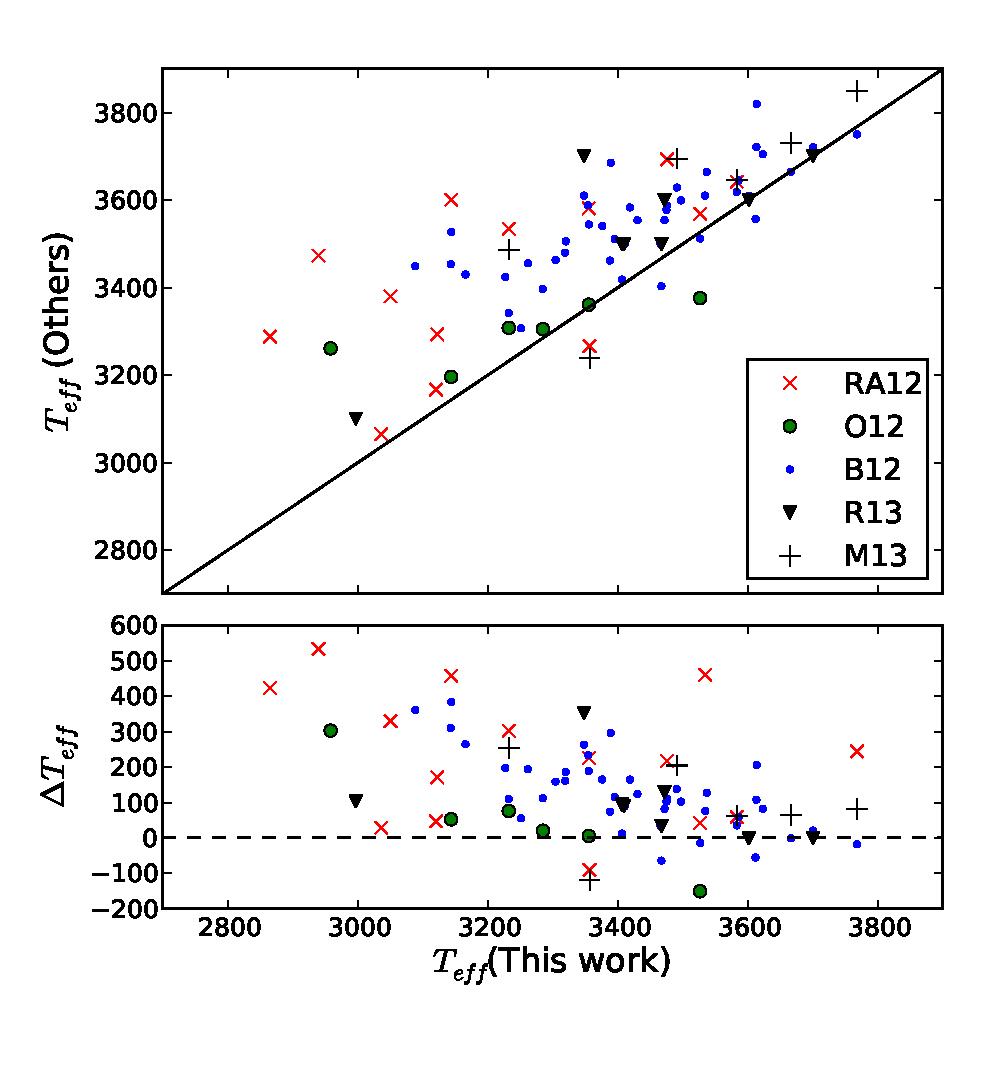
\includegraphics[scale=0.5]{pics/compteff.eps}
\end{center}
\caption{\textit{Upper panel:} $T_{eff}$-$T_{eff}$ plot comparing the values of this work against others in the literature. The solid black line depicts the identity line;\textit{Lower panel:} Comparison plot residuals. The dashed black line marks the zero point of our calibration.}
\label{fig:compteff}
\end{figure}

We also calculated linear fits for the three $T_{eff}$ scales of BO12, RA12, and R13 where we consider we have enough stars in common. For the BO12 the relation is

\begin{equation}
T_{eff} = (1.078\pm0.144) T_{eff,B12} - 401.961\pm511.704,
\end{equation}
for RA12,
\begin{equation}
T_{eff} = (0.731\pm0.176) T_{eff,RA12} + 712.216\pm617.706,
\end{equation}
and for R13,
\begin{equation}
T_{eff} = (1.106\pm0.158) T_{eff,R13} - 481.857\pm545.780
\end{equation}

The photometric [Fe/H] measurements as well as the $T_{eff}$ determinations using the calibration of B12 were calculated with the data from Table \ref{table:params}. 

For metallicity we observe a general agreement between our results and the ones from the literature. We note here that the calibration of SL10 is very similar to our reference calibration, from \citet{Neves-2012}, and this is the reason why we obtain a value of dispersion smaller than the one of the original calibration (0.11 vs 0.17 dex). The dispersion of the oldest photometric calibration B05 is surprisingly low, considering that the original dispersion for this calibration is 0.20 dex. Regarding the J12 calibration, we obtain a $rms$ of 0.20 dex, higher that their reported value of 0.15 dex. The dispersion of the spectroscopic calibrations are within the expected values (0.12 dex). The offset is smaller than the dispersion value of our calibration. We combined all spectroscopic calibrations due to a lack of stars in common but we also show the results of RA12 separately, where we have 15 data points. 

\textbf{Regarding $T_{eff}$ we observe a good agreement with the latest results from R13 using the latest BT-SETTL models. In fact, if we remove the outlier star GJ 382, we obtain a $rms$ of 116 K and an offset of 87 K, practically within the uncertainties of the R13 determinations. However we also observe considerable dispersion and offset with both RA12 and BO12 comparison samples. The BO12 determination tend to converge with ours as the $T_{eff}$ increases. %The M13b values, on the other hand, show an increasing systematic overestimation of the $T_{eff}$ for values higher than 3400 K. 
We also note a systematic underestimation of our values of temperature in general that increases below 3200K. The O12 determinations have the smallest scatter and offset, but this result is expected since they use the same reference $T_{eff}$ calibration as we do.}

\subsection{Using the calibration}

The code of the calibration is written in python 2.7 and can be downloaded at \url{http://www.astro.up.pt/resources/mcal}. The program is very simple to use. The first step is to write the filenames of your spectra into \textit{stars.txt}, replacing the two demonstration filenames, \textit{Gl105B\_ S1D.fits} and \textit{Gl849\_ S1D.fits}. Then, one just need to change the startup options, described in the startup section of the file \textit{runallv1.py}. Depending on the resolution and SNR of the spectra, one should use the values of Table \ref{table:snres} as the reference of precision of [Fe/H] and $T_{eff}$.

The compressed zip file \textit{calibration.zip} contains all the necessary files needed to run the calibration, as described in the following list:
\begin{itemize}
\item \textit{runallv1.py} - script to run all the other programs. In the startup section one can choose to use FFT to filter high frequency noise, the file type of the input spectra (FITS or text file), and the name of the file with the full path of the spectra.
\item \textit{fft\_ filterv1.py} - function that performs the FFT filtering of the spectra.  It takes 5-10 minutes per star to use this filter depending on CPU processing power.
\item \textit{int\_ calc\_ stars.py} - function to calculate the pseudo EWs of the relevant lines. It uses lines.rdb as input. An output file, ew\_ out.npz, is also created. It takes 3-5 minutes per star to calculate the EWs.
\item \textit{mcalv1.npz} - function that calculates the [Fe/H] and Teff of each star using the calibration matrix file \textit{coef\_ cal.npz}. the output will be displayed on the screen and can also be optionally saved to a file (check the startup section of \textit{runallv1.py} for details). 
\item \textit{stars.txt} - text file with the full path of the spectra. This file should have all the spectra files for analysis.
\item \textit{Gl105B\_ S1D.fits} and \textit{Gl849\_ S1D.fits} are two HARPS spectra that can be used to demonstrate how the program works. Their full file names appear in the file stars.txt. One should remove them from \textit{stars.txt} before calibrating new stars.
\end{itemize}

 %We also note an increasing disagreement with BO12 with decreasing temperature for $T_{eff} < 3000$ K. 




\section{Discussion}
\label{sec:discussion}

In this paper we present a new high-precision calibration for M dwarfs. We achieve a $rms$ of 0.07 dex for metallicity and 100 K for effective temperature. Alternatively we obtain a RMSE$_{V}$ value of 0.08 dex for [Fe/H] and 300 K for $T_{eff}$. A bootstrap resampling was also conducted, showing a variation of the $rms$ of [Fe/H] and $T_{eff}$ of the order of $\pm$ 0.01 dex and $\pm$ 20 K respectively. Our calibration is available for download at \url{http://www.astro.up.pt/resources/mcal}. The procedure to use our calibration is detailed in this webpage. A test of the performance of the calibration as a function of the resolution and SNR was also performed. We conclude that the calibration behaves well down to R = 50.000 and SNR = 25, after correcting the observed trends. 

%but consider that the offset must be corrected in all cases, due to the nature of the `peak-to-peak' technique that does not account for the continuum.  

To have a measure of the accuracy of our calibration, we tested it against several studies from the literature. Most studies agree well with our [Fe/H] determinations, and the offset is almost always below the precision of the calibration. For $T_{eff}$ however, the same agreement could not be met. Despite reaching a very good agreement with the results of \citet{Rajpurohit-2013a}, that use synthetic spectra from the latest BT-SETTL models, the dispersion as well as the systematics between our calibration and the other works is considerable and beyond the calibration errors. Further studies are needed to investigate the nature of these systematics. 

%A companion paper, Neves et al. (in prep.), using the same technique but anchored in metallicity values taken from FGK primaries with a M dwarf secondary is being finalised and will be submitted soon. \textcolor{red}{more details about this paper?}




%Expansion to other elements, activity, vsini...

%We suggest that, further to the present paper, the users cite the parameter sources in case if a star-by-star analysis.




\begin{acknowledgements}
We acknowledge the support by the European Research Council/European Community under the FP7 through Starting Grant agreement number 239953. The financial support from the "Programme National de Plan\'etologie'' (PNP) of CNRS/INSU, France, is gratefully acknowledged. VN acknowledges the support from Funda\c{c}\~ao para a Ci\^encia e a Tecnologia (FCT) of the fellowship SFRH/BD/60688/2009. NCS also acknowledges the support in the form of a Investigador FCT contract funded by Funda\c{c}\~ao para a Ci\^encia e a Tecnologia (FCT) /MCTES (Portugal) and POPH/FSE (EC). This research has made use of the SIMBAD database, operated at CDS, Strasbourg, France, and of the Extrasolar Planet Encyclopaedia at ~ \url{exoplanet.eu}. This publication makes use of data products from the Two Micron All Sky Survey, which is a joint project of the University of Massachusetts and the Infrared Processing and Analysis Center/California Institute of Technology, funded by the National Aeronautics and Space Administration and the National Science Foundation.

\end{acknowledgements}

\bibliographystyle{aa}
\bibliography{mylib}




\end{document}

####bib references!!!



%%%%%%%%%%%%%%%%%%%%%%%%%%%%%%%%%%%%%%%%%%%%%%%%%%%%%%%%%%%%%%
Examples for figures using graphicx
A guide "Using Imported Graphics in LaTeX2e"  (Keith Reckdahl)
is available on a lot of LaTeX public servers or ctan mirrors.
The file is : epslatex.pdf 
%%%%%%%%%%%%%%%%%%%%%%%%%%%%%%%%%%%%%%%%%%%%%%%%%%%%%%%%%%%%%%

%_____________________________________________________________
%                 A figure as large as the width of the column
%-------------------------------------------------------------
   \begin{figure}
   \centering
   \includegraphics[width=\hsize]{empty.eps}
      \caption{Vibrational stability equation of state
               $S_{\mathrm{vib}}(\lg e, \lg \rho)$.
               $>0$ means vibrational stability.
              }
         \label{FigVibStab}
   \end{figure}
%
%_____________________________________________________________
%                                    One column rotated figure
%-------------------------------------------------------------
   \begin{figure}
   \centering
   \includegraphics[angle=-90,width=3cm]{empty.eps}
      \caption{Vibrational stability equation of state
               $S_{\mathrm{vib}}(\lg e, \lg \rho)$.
               $>0$ means vibrational stability.
              }
         \label{FigVibStab}
   \end{figure}
%
%_____________________________________________________________
%                        Figure with caption on the right side 
%-------------------------------------------------------------
   \begin{figure}
   \sidecaption
   \includegraphics[width=3cm]{empty.eps}
      \caption{Vibrational stability equation of state
               $S_{\mathrm{vib}}(\lg e, \lg \rho)$.
               $>0$ means vibrational stability.
              }
         \label{FigVibStab}
   \end{figure}
%
%_____________________________________________________________
%
%_____________________________________________________________
%                                Figure with a new BoundingBox 
%-------------------------------------------------------------
   \begin{figure}
   \centering
   \includegraphics[bb=10 20 100 300,width=3cm,clip]{empty.eps}
      \caption{Vibrational stability equation of state
               $S_{\mathrm{vib}}(\lg e, \lg \rho)$.
               $>0$ means vibrational stability.
              }
         \label{FigVibStab}
   \end{figure}
%
%_____________________________________________________________
%
%_____________________________________________________________
%                                      The "resizebox" command 
%-------------------------------------------------------------
   \begin{figure}
   \resizebox{\hsize}{!}
            {\includegraphics[bb=10 20 100 300,clip]{empty.eps}
      \caption{Vibrational stability equation of state
               $S_{\mathrm{vib}}(\lg e, \lg \rho)$.
               $>0$ means vibrational stability.
              }
         \label{FigVibStab}
   \end{figure}
%
%______________________________________________________________
%
%_____________________________________________________________
%                                             Two column Figure 
%-------------------------------------------------------------
   \begin{figure*}
   \resizebox{\hsize}{!}
            {\includegraphics[bb=10 20 100 300,clip]{empty.eps}
      \caption{Vibrational stability equation of state
               $S_{\mathrm{vib}}(\lg e, \lg \rho)$.
               $>0$ means vibrational stability.
              }
         \label{FigVibStab}
   \end{figure*}
%
%______________________________________________________________
%
%_____________________________________________________________
%                                             Simple A&A Table
%_____________________________________________________________
%
\begin{table}
\caption{Nonlinear Model Results}             % title of Table
\label{table:1}      % is used to refer this table in the text
\centering                          % used for centering table
\begin{tabular}{c c c c}        % centered columns (4 columns)
\hline\hline                 % inserts double horizontal lines
HJD & $E$ & Method\#2 & Method\#3 \\    % table heading 
\hline                        % inserts single horizontal line
   1 & 50 & $-837$ & 970 \\      % inserting body of the table
   2 & 47 & 877    & 230 \\
   3 & 31 & 25     & 415 \\
   4 & 35 & 144    & 2356 \\
   5 & 45 & 300    & 556 \\ 
\hline                                   %inserts single line
\end{tabular}
\end{table}
%
%_____________________________________________________________
%                                             Two column Table 
%_____________________________________________________________
%
\begin{table*}
\caption{Nonlinear Model Results}             
\label{table:1}      
\centering          
\begin{tabular}{c c c c l l l }     % 7 columns 
\hline\hline       
                      % To combine 4 columns into a single one 
HJD & $E$ & Method\#2 & \multicolumn{4}{c}{Method\#3}\\ 
\hline                    
   1 & 50 & $-837$ & 970 & 65 & 67 & 78\\  
   2 & 47 & 877    & 230 & 567& 55 & 78\\
   3 & 31 & 25     & 415 & 567& 55 & 78\\
   4 & 35 & 144    & 2356& 567& 55 & 78 \\
   5 & 45 & 300    & 556 & 567& 55 & 78\\
\hline                  
\end{tabular}
\end{table*}
%
%-------------------------------------------------------------
%                                          Table with notes 
%-------------------------------------------------------------
%
% A single note
\begin{table}
\caption{\label{t7}Spectral types and photometry for stars in the
  region.}
\centering
\begin{tabular}{lccc}
\hline\hline
Star&Spectral type&RA(J2000)&Dec(J2000)\\
\hline
69           &B1\,V     &09 15 54.046 & $-$50 00 26.67\\
49           &B0.7\,V   &*09 15 54.570& $-$50 00 03.90\\
LS~1267~(86) &O8\,V     &09 15 52.787&11.07\\
24.6         &7.58      &1.37 &0.20\\
\hline
LS~1262      &B0\,V     &09 15 05.17&11.17\\
MO 2-119     &B0.5\,V   &09 15 33.7 &11.74\\
LS~1269      &O8.5\,V   &09 15 56.60&10.85\\
\hline
\end{tabular}
\tablefoot{The top panel shows likely members of Pismis~11. The second
panel contains likely members of Alicante~5. The bottom panel
displays stars outside the clusters.}
\end{table}
%
% More notes
%
\begin{table}
\caption{\label{t7}Spectral types and photometry for stars in the
  region.}
\centering
\begin{tabular}{lccc}
\hline\hline
Star&Spectral type&RA(J2000)&Dec(J2000)\\
\hline
69           &B1\,V     &09 15 54.046 & $-$50 00 26.67\\
49           &B0.7\,V   &*09 15 54.570& $-$50 00 03.90\\
LS~1267~(86) &O8\,V     &09 15 52.787&11.07\tablefootmark{a}\\
24.6         &7.58\tablefootmark{1}&1.37\tablefootmark{a}   &0.20\tablefootmark{a}\\
\hline
LS~1262      &B0\,V     &09 15 05.17&11.17\tablefootmark{b}\\
MO 2-119     &B0.5\,V   &09 15 33.7 &11.74\tablefootmark{c}\\
LS~1269      &O8.5\,V   &09 15 56.60&10.85\tablefootmark{d}\\
\hline
\end{tabular}
\tablefoot{The top panel shows likely members of Pismis~11. The second
panel contains likely members of Alicante~5. The bottom panel
displays stars outside the clusters.\\
\tablefoottext{a}{Photometry for MF13, LS~1267 and HD~80077 from
Dupont et al.}
\tablefoottext{b}{Photometry for LS~1262, LS~1269 from
Durand et al.}
\tablefoottext{c}{Photometry for MO2-119 from
Mathieu et al.}
}
\end{table}
%
%-------------------------------------------------------------
%                                       Table with references 
%-------------------------------------------------------------
%
\begin{table*}[h]
 \caption[]{\label{nearbylistaa2}List of nearby SNe used in this work.}
\begin{tabular}{lccc}
 \hline \hline
  SN name &
  Epoch &
 Bands &
  References \\
 &
  (with respect to $B$ maximum) &
 &
 \\ \hline
1981B   & 0 & {\it UBV} & 1\\
1986G   &  $-$3, $-$1, 0, 1, 2 & {\it BV}  & 2\\
1989B   & $-$5, $-$1, 0, 3, 5 & {\it UBVRI}  & 3, 4\\
1990N   & 2, 7 & {\it UBVRI}  & 5\\
1991M   & 3 & {\it VRI}  & 6\\
\hline
\noalign{\smallskip}
\multicolumn{4}{c}{ SNe 91bg-like} \\
\noalign{\smallskip}
\hline
1991bg   & 1, 2 & {\it BVRI}  & 7\\
1999by   & $-$5, $-$4, $-$3, 3, 4, 5 & {\it UBVRI}  & 8\\
\hline
\noalign{\smallskip}
\multicolumn{4}{c}{ SNe 91T-like} \\
\noalign{\smallskip}
\hline
1991T   & $-$3, 0 & {\it UBVRI}  &  9, 10\\
2000cx  & $-$3, $-$2, 0, 1, 5 & {\it UBVRI}  & 11\\ %
\hline
\end{tabular}
\tablebib{(1)~\citet{branch83};
(2) \citet{phillips87}; (3) \citet{barbon90}; (4) \citet{wells94};
(5) \citet{mazzali93}; (6) \citet{gomez98}; (7) \citet{kirshner93};
(8) \citet{patat96}; (9) \citet{salvo01}; (10) \citet{branch03};
(11) \citet{jha99}.
}
\end{table}
%_____________________________________________________________
%                      A rotated Two column Table in landscape  
%-------------------------------------------------------------
\begin{sidewaystable*}
\caption{Summary for ISOCAM sources with mid-IR excess 
(YSO candidates).}\label{YSOtable}
\centering
\begin{tabular}{crrlcl} 
\hline\hline             
ISO-L1551 & $F_{6.7}$~[mJy] & $\alpha_{6.7-14.3}$ 
& YSO type$^{d}$ & Status & Comments\\
\hline
  \multicolumn{6}{c}{\it New YSO candidates}\\ % To combine 6 columns into a single one
\hline
  1 & 1.56 $\pm$ 0.47 & --    & Class II$^{c}$ & New & Mid\\
  2 & 0.79:           & 0.97: & Class II ?     & New & \\
  3 & 4.95 $\pm$ 0.68 & 3.18  & Class II / III & New & \\
  5 & 1.44 $\pm$ 0.33 & 1.88  & Class II       & New & \\
\hline
  \multicolumn{6}{c}{\it Previously known YSOs} \\
\hline
  61 & 0.89 $\pm$ 0.58 & 1.77 & Class I & \object{HH 30} & Circumstellar disk\\
  96 & 38.34 $\pm$ 0.71 & 37.5& Class II& MHO 5          & Spectral type\\
\hline
\end{tabular}
\end{sidewaystable*}
%_____________________________________________________________
%                      A rotated One column Table in landscape  
%-------------------------------------------------------------
\begin{sidewaystable}
\caption{Summary for ISOCAM sources with mid-IR excess 
(YSO candidates).}\label{YSOtable}
\centering
\begin{tabular}{crrlcl} 
\hline\hline             
ISO-L1551 & $F_{6.7}$~[mJy] & $\alpha_{6.7-14.3}$ 
& YSO type$^{d}$ & Status & Comments\\
\hline
  \multicolumn{6}{c}{\it New YSO candidates}\\ % To combine 6 columns into a single one
\hline
  1 & 1.56 $\pm$ 0.47 & --    & Class II$^{c}$ & New & Mid\\
  2 & 0.79:           & 0.97: & Class II ?     & New & \\
  3 & 4.95 $\pm$ 0.68 & 3.18  & Class II / III & New & \\
  5 & 1.44 $\pm$ 0.33 & 1.88  & Class II       & New & \\
\hline
  \multicolumn{6}{c}{\it Previously known YSOs} \\
\hline
  61 & 0.89 $\pm$ 0.58 & 1.77 & Class I & \object{HH 30} & Circumstellar disk\\
  96 & 38.34 $\pm$ 0.71 & 37.5& Class II& MHO 5          & Spectral type\\
\hline
\end{tabular}
\end{sidewaystable}
%
%_____________________________________________________________
%                              Table longer than a single page  
%-------------------------------------------------------------
% All long tables will be placed automatically at the end, after 
%                                        \end{thebibliography}
%
\begin{longtab}
\begin{longtable}{lllrrr}
\caption{\label{kstars} Sample stars with absolute magnitude}\\
\hline\hline
Catalogue& $M_{V}$ & Spectral & Distance & Mode & Count Rate \\
\hline
\endfirsthead
\caption{continued.}\\
\hline\hline
Catalogue& $M_{V}$ & Spectral & Distance & Mode & Count Rate \\
\hline
\endhead
\hline
\endfoot
%%
Gl 33    & 6.37 & K2 V & 7.46 & S & 0.043170\\
Gl 66AB  & 6.26 & K2 V & 8.15 & S & 0.260478\\
Gl 68    & 5.87 & K1 V & 7.47 & P & 0.026610\\
         &      &      &      & H & 0.008686\\
Gl 86 
\footnote{Source not included in the HRI catalog. See Sect.~5.4.2 for details.}
         & 5.92 & K0 V & 10.91& S & 0.058230\\
\end{longtable}
\end{longtab}
%
%_____________________________________________________________
%                              Table longer than a single page
%                                             and in landscape 
%  In the preamble, use:       \usepackage{lscape}
%-------------------------------------------------------------
% All long tables will be placed automatically at the end, after
%                                        \end{thebibliography}
%
\begin{longtab}
\begin{landscape}
\begin{longtable}{lllrrr}
\caption{\label{kstars} Sample stars with absolute magnitude}\\
\hline\hline
Catalogue& $M_{V}$ & Spectral & Distance & Mode & Count Rate \\
\hline
\endfirsthead
\caption{continued.}\\
\hline\hline
Catalogue& $M_{V}$ & Spectral & Distance & Mode & Count Rate \\
\hline
\endhead
\hline
\endfoot
%%
Gl 33    & 6.37 & K2 V & 7.46 & S & 0.043170\\
Gl 66AB  & 6.26 & K2 V & 8.15 & S & 0.260478\\
Gl 68    & 5.87 & K1 V & 7.47 & P & 0.026610\\
         &      &      &      & H & 0.008686\\
Gl 86
\footnote{Source not included in the HRI catalog. See Sect.~5.4.2 for details.}
         & 5.92 & K0 V & 10.91& S & 0.058230\\
\end{longtable}
\end{landscape}
\end{longtab}
%
% Online Material
%_____________________________________________________________
%        Online appendices have to be placed at the end, after
%                                        \end{thebibliography}
%-------------------------------------------------------------
\end{thebibliography}

\Online

\begin{appendix} %First online appendix
\section{Background galaxy number counts and shear noise-levels}
Because the optical images used in this analysis...

\begin{figure*}
\centering
\includegraphics[width=16.4cm,clip]{1787f24.ps}
\caption{Plotted above...}
\label{appfig}
\end{figure*}

Because the optical images...
\end{appendix}

\begin{appendix} %Second online appendix
These studies, however, have faced...
\end{appendix}

\end{document}
%
%_____________________________________________________________
%        Some tables or figures are in the printed version and
%                      some are only in the electronic version
%-------------------------------------------------------------
%
% Leave all the tables or figures in the text, at their right place 
% and use the commands \onlfig{} and \onltab{}. These elements
% will be automatically placed at the end, in the section
% Online material.

\documentclass{aa}
...
\begin{document}
text of the paper...
\begin{figure*}%f1
\includegraphics[width=10.9cm]{1787f01.eps}
\caption{Shown in greyscale is a...}
\label{cl12301}}
\end{figure*}
...
from the intrinsic ellipticity distribution.
% Figure 2 available electronically only
\onlfig{
\begin{figure*}%f2
\includegraphics[width=11.6cm]{1787f02.eps}
\caption {Shown in greyscale...}
\label{cl1018}
\end{figure*}
}

% Figure 3 available electronically only
\onlfig{
\begin{figure*}%f3
\includegraphics[width=11.2cm]{1787f03.eps}
\caption{Shown in panels...}
\label{cl1059}
\end{figure*}
}

\begin{figure*}%f4
\includegraphics[width=10.9cm]{1787f04.eps}
\caption{Shown in greyscale is...}
\label{cl1232}}
\end{figure*}

\begin{table}%t1
\caption{Complexes characterisation.}\label{starbursts}
\centering
\begin{tabular}{lccc}
\hline \hline
Complex & $F_{60}$ & 8.6 &  No. of  \\
...
\hline
\end{tabular}
\end{table}
The second method produces...

% Figure 5 available electronically only
\onlfig{
\begin{figure*}%f5
\includegraphics[width=11.2cm]{1787f05.eps}
\caption{Shown in panels...}
\label{cl1238}}
\end{figure*}
}

As can be seen, in general the deeper...
% Table 2 available electronically only
\onltab{
\begin{table*}%t2
\caption{List of the LMC stellar complexes...}\label{Properties}
\centering
\begin{tabular}{lccccccccc}
\hline  \hline
Stellar & RA & Dec & ...
...
\hline
\end{tabular}
\end{table*}
}

% Table 3 available electronically only
\onltab{
\begin{table*}%t3
\caption{List of the derived...}\label{IrasFluxes}
\centering
\begin{tabular}{lcccccccccc}
\hline \hline
Stellar & $f12$ & $L12$ &...
...
\hline
\end{tabular}
\end{table*}
}
%
%-------------------------------------------------------------
%     For the online material, table longer than a single page
%                 In the preamble for landscape case, use : 
%                                          \usepackage{lscape}
%-------------------------------------------------------------
\documentclass{aa}
\usepackage[varg]{txfonts}
\usepackage{graphicx}
\usepackage{lscape}

\begin{document}
text of the paper
% Table will be print automatically at the end, in the section Online material.
\onllongtab{
\begin{longtable}{lrcrrrrrrrrl}
\caption{Line data and abundances ...}\\
\hline
\hline
Def & mol & Ion & $\lambda$ & $\chi$ & $\log gf$ & N & e &  rad & $\delta$ & $\delta$ 
red & References \\
\hline
\endfirsthead
\caption{Continued.} \\
\hline
Def & mol & Ion & $\lambda$ & $\chi$ & $\log gf$ & B & C &  rad & $\delta$ & $\delta$ 
red & References \\
\hline
\endhead
\hline
\endfoot
\hline
\endlastfoot
A & CH & 1 &3638 & 0.002 & $-$2.551 &  &  &  & $-$150 & 150 &  Jorgensen et al. (1996) \\                    
\end{longtable}
}% End onllongtab

% Or for landscape, large table:

\onllongtab{
\begin{landscape}
\begin{longtable}{lrcrrrrrrrrl}
...
\end{longtable}
\end{landscape}
}% End onllongtab
